\documentclass[10pt,a4paper,UTF8]{ctexart}

\linespread{1.5}
\usepackage{geometry}%用于设置上下左右页边距
	\geometry{left=2.5cm,right=2.5cm,top=3.2cm,bottom=2.7cm}
\usepackage{xeCJK,amsmath,paralist,enumerate,booktabs,multirow,graphicx,subfig,setspace,listings,lastpage,hyperref}
\usepackage{amsthm, amssymb, bm, color, framed, graphicx, hyperref, mathrsfs}
\usepackage{mathrsfs}  
	\setlength{\parindent}{2em}
	\lstset{language=Matlab}%
\usepackage{fancyhdr}
\usepackage{graphicx}
\usepackage{subfloat}
\usepackage{listings}
\usepackage{xcolor}
\usepackage{float}
\usepackage{paralist}
\usepackage{setspace}
\usepackage{titlesec}
\usepackage{enumitem}
\usepackage{hyperref}
\usepackage{multirow}
\usepackage{threeparttable}
\usepackage{tcolorbox}
\usepackage{tabularx}
\usepackage{ulem}
\usepackage{longtable}
\usepackage{multicol}
\usepackage{pifont}
\usepackage{lipsum}
\usepackage{microtype}
\usepackage{wrapfig}
\usepackage[absolute,overlay]{textpos}
\usepackage{makecell}

\hypersetup{
	colorlinks=true,
	linkcolor=black
}

\setenumerate{partopsep=0pt,topsep=0pt,itemsep=-2pt,leftmargin=2em}
\setitemize{itemsep=-2pt,partopsep=0pt,topsep=0pt,leftmargin=2em}

\titlespacing*{\section}{0pt}{3pt}{3pt}
\titlespacing*{\subsection}{0pt}{2pt}{2pt}
\titlespacing*{\subsubsection}{0pt}{1pt}{1pt}
\titlespacing*{\paragraph}{0pt}{0pt}{0pt}

\ctexset{secnumdepth=4,tocdepth=4}
\setlength{\parindent}{0pt}
\setstretch{1.35}


\setCJKmainfont[BoldFont={FZHei-B01},ItalicFont={FZKai-Z03}]{FZShuSong-Z01} 
\setCJKsansfont[BoldFont={FZHei-B01}]{FZKai-Z03} 
\setCJKmonofont[BoldFont={FZHei-B01}]{FZFangSong-Z02}
\setCJKfamilyfont{zhsong}{FZShuSong-Z01} 
\setCJKfamilyfont{zhhei}{FZHei-B01} 
\setCJKfamilyfont{zhkai}[BoldFont={FZHei-B01}]{FZKai-Z03} 
\setCJKfamilyfont{zhfs}[BoldFont={FZHei-B01}]{FZFangSong-Z02} 
\renewcommand*{\songti}{\CJKfamily{zhsong}} 
\renewcommand*{\heiti}{\CJKfamily{zhhei}} 
\renewcommand*{\kaishu}{\CJKfamily{zhkai}} 
\renewcommand*{\fangsong}{\CJKfamily{zhfs}}


\definecolor{mKeyword}{RGB}{0,0,255}          % bule
\definecolor{mString}{RGB}{160,32,240}        % purple
\definecolor{mComment}{RGB}{34,139,34}        % green
\definecolor{mNumber}{RGB}{128,128,128} 

\lstdefinestyle {njulisting} {
	basewidth = 0.5 em,
	lineskip = 3 pt,
	basicstyle = \small\ttfamily,
	% keywordstyle = \bfseries,
	commentstyle = \itshape\color{gray}, 
	basicstyle=\small\ttfamily,
	keywordstyle={\color{mKeyword}},     % sets color for keywords
	stringstyle={\color{mString}},       % sets color for strings
	commentstyle={\color{mComment}},     % sets color for comments
	numberstyle=\tiny\color{mNumber},
	numbers = left,
	captionpos = t,
	breaklines = true,
	xleftmargin = 1 em,
	xrightmargin = 0 em,
	frame=tlrb,
	tabsize=4
}

\lstset{
style = njulisting, % 调用上述样式 
flexiblecolumns % 允许调整字符宽度
}


%================= 基本格式预置 ===========================
\usepackage{fancyhdr}
\pagestyle{fancy}
\lhead{\textsc{SOA and Software Engineering}}
\rhead{面向服务的软件工程}
\cfoot{\thepage}
\renewcommand{\headrulewidth}{0.4pt}
\renewcommand{\theenumi}{(\arabic{enumi})}
\CTEXsetup[format={\bfseries\zihao{-3}}]{section}
\CTEXsetup[format={\bfseries\zihao{4}}]{subsection}
\CTEXsetup[format={\bfseries\zihao{-4}}]{subsubsection}


\renewcommand{\contentsname}{目录}  

%\definecolor{shadecolor}{RGB}{241, 241, 255}
\newcounter{problemname}
\newenvironment{problem}{\stepcounter{problemname}\par\noindent\textbf{\arabic{problemname}.\,} \kaishu}{}
\newenvironment{solution}{}{\vspace{0.25em}}

\newcommand{\myline}{\uline{\ \ \ \ \ \ \ \ \ \ }}

\begin{document}
	\begin{center}
		\LARGE\textbf{面向服务的软件工程简答题整理}
	\end{center}

	\setlength{\parskip}{0.25em}

	\begin{problem}
    制造与服务的区别?
    \end{problem}
    
    \begin{solution}
    \begin{spacing}{1.25}
        \begin{longtable}{|W{c}{1.8cm}|m{6.4cm}|m{6.2cm}|}
            \hline
            \multicolumn{1}{|c|}{\textbf{}} & \multicolumn{1}{c|}{\textbf{制造}} & \multicolumn{1}{c|}{\textbf{服务}} \\ \hline
            物质性 & 产品是可以被实体触摸的有形物品 & 服务是无形的,不能被实体触摸 \\ \hline
            交付方式 & 产品通常以物理形式交付 & 服务通过可远程访问的接口交付 \\ \hline
            寿命 & 产品有一个固定的寿命,通常使用到磨损或过时 & 服务可以重复使用,并且随着时间的推移可能会被更新或修改 \\ \hline
            定制 & 产品通常是大量生产的,不能轻易定制 & 服务可以根据客户的需求进行定制 \\ \hline
            价值 & 产品通常基于其特征和质量进行估值 & 服务则基于其满足特定需求或解决特定问题的能力进行估值 \\ \hline
        \end{longtable}
        \vspace{-1em}
    \end{spacing}
    
    商品与服务的精确定义应根据其属性加以区分
    \begin{itemize}
        \item 商品是可以创造和转让的有形实物或产品;它随着时间的推移而存在,因此可以在以后创建和使用。
        \item 服务是无形的,易变质的。它是同时或几乎同时创建和使用的事件或过程。虽然消费者在实际服务产生后无法保留,但服务的努力可以保留。
    \end{itemize}
    \end{solution}
	\begin{problem}
    为何需要构建服务生态系统?什么是服务生态系统中的垂直服务和水平服务?它们有何联系和区别?试举例加以说明。
    \end{problem}
    
    \begin{solution}
    服务生态系统是一种由多个互相依赖和交互的服务组成的系统,其目的是为了满足不同用户和应用程序的需求。它可以帮助企业和组织构建完整的解决方案,提高效率和降低成本。
    
    为何需要构建服务生态系统:
    \begin{itemize}
        \item 一方面,面向服务的快速发展导致单个组织无法独立提供全套服务,提供的有限服务也无法被广泛运用;已存在的服务并不能很好的被发现和调用,也导致了大量冗余服务
        \item 另一方面,原先的服务系统是复杂、脆弱、特殊的,从上层业务看,无法灵活应对实际业务的变更;从底层实现看,也无法及时应对底层技术的更新、或者新增的功能
        \item 因此构建服务生态系统,运用面向服务的分析和设计原则,使得产生的服务具有良好的可发现性和可复用性,同时能灵活应对业务领域和技术领域的变更
    \end{itemize}
    
    \begin{spacing}{1.2}
        \vspace{-0.5em}
        \begin{longtable}{|m{7.5cm}|m{7.5cm}|}
            \hline
            \multicolumn{1}{|c|}{\textbf{垂直服务}} & \multicolumn{1}{c|}{\textbf{水平服务}} \\ \hline
            \vspace{-1.3em}
            \begin{itemize}[leftmargin=1.5em,itemsep=-3pt]
                \item 单独面向一个客户,提供系列功能的服务
                \item 从消费者的角度说,垂直服务可以被同时、独立地使用,分为纯IT服务和IT使能的服务
            \vspace{-1.5em}
            \end{itemize}                                           
                & 
            \vspace{-1.3em}
            \begin{itemize}[leftmargin=1.5em,itemsep=-3pt]
                \item 用于构建垂直服务、可重用的、跨行业的公共服务
                \item 分为公共业务服务和IT服务
            \vspace{-1.5em}
            \end{itemize}  
            \\ \hline
        \end{longtable}
        \vspace{-1em}
    \end{spacing}
    
    
    垂直服务和水平服务的联系与区别:
    \begin{itemize}
        \item 垂直服务和水平服务都是通过服务系统来实现业务服务
        \item 水平服务是功能相关的,简单且相对稳定,一般由IT专家开发
        \item 垂直服务是流程相关的,复杂且易变更,需要领域专家参与开发
        \item 垂直服务实际上是一系列水平服务的封装,将上下文无关的水平服务根据特定的业务流程进行编排,最后打包为一个解决特定问题的垂直服务
    \end{itemize}
    
    举例:
    学校的借书服务、打印成绩单服务是垂直服务,都需要进行身份认证,身份认证就是一个水平服务;借书服务和打印成绩单服务除了身份认证还包含其他的服务,就是将简单的水平服务构建成能实现业务目标或流程的垂直服务
    \end{solution}
	\begin{problem}
对比面向服务的范型和面向服务的范型
\end{problem}

\begin{solution}
\begin{spacing}{1.2}
    \centering
    \begin{longtable}{|m{1.8cm}<{\centering}|m{6.5cm}|m{6.5cm}|}
		\hline
    \textbf{特点} & \multicolumn{1}{c|}{\textbf{面向对象的计算}}                   & \multicolumn{1}{c|}{\textbf{面向服务计算}}                                                          \\ \hline
    方法论         & 通过定义紧耦合的类来进行应用开发;应用架构为基于继承关系的层次式架构;从构造函数——通过类或模型——到系统设计 & 通过定义松耦合的服务来进行应用开发,并将服务组装成可执行的应用;从系统模型到服务模块,从服务抽象定义到服务实现绑定;通过搜索获得可用的服务实现                       \\ \hline
    抽象和协作层次     & 往往由一个团队来负责应用的开发,并负责整个生命周期;开发者必须了解应用领域知识和编程              & 开发任务由三个独立方承担:应用程序开发者,服务提供方和服务代理;其中,应用程序开发者需要了解应用逻辑,但不需要了解具体的服务是如何实现的;服务提供者需要编程能力,但不必了解使用服务的应用 \\ \hline
    代码共享和复用     & 代码复用通过类成员的继承和库函数加以实现。其中库函数在编译时引入,且往往是平台相关的              & 代码在服务层次复用。服务使用标准的结构,并发布在Internet库中。服务是平台无关的,且能够被查找并远程调用。服务代理支持系统的服务共享                         \\ \hline
    动态绑定和重新组合   & 在运行时将名称和方法进行关联。方法必须在应用部署前链接到可执行的代码                      & 在运行时将服务调用和服务进行绑定。可以在应用部署后,再进行服务选定。这一特色使得应用可以在运行时重组                                            \\ \hline
    重组          & 多在设计时决定导入的组件                                            & 可以动态改变应用系统中服务的组合关系,以及服务定义与服务实现之间的绑定关系,即实现动态地添加、修改、删除各个服务节点                                    \\ \hline
    组件通讯和接口     & 与平台和语言有关,例如C++程序难以直接和Java程序通信                           & 与平台和语言无关。组件间通过标准协议通信,如XML,WSDL和SOAP                                                           \\ \hline
    系统维护        & 用户需要时常升级软件,且在执行升级时,应用必须停止                               & 通过互联网升级系统,因为服务多运行在远程服务器上,用户通过互联网进行访问。维护对用户透明                                                  \\ \hline
    可靠性         & 在设计时决定可靠性的方法                                            & 对于服务提供者,每个服务相对简单,更加可靠。对于应用程序存在多个满足同一需求的服务,可用过将故障服务的节点断开并重新绑定到备选服务节点上,获得不间断的应用系统               \\ \hline
    软件拥有        & 软件作为产品销售,为用户所拥有                                         & 软件存在并执行于独立的服务提供商的设备上,用户按照每次对服务使用付费,而不是按照软件产品付费                                                \\ \hline
    \end{longtable}
	\end{spacing}
\vspace{-1em}


从设计角度和实现角度来看
\vspace{-0.5em}
\begin{spacing}{1.2}
    \centering
    \begin{longtable}{|m{1.2cm}<{\centering}|m{6.7cm}|m{6.7cm}|}
        \hline
\textbf{特点} & \multicolumn{1}{c|}{\textbf{面向对象的计算}} & \multicolumn{1}{c|}{\textbf{面向服务计算}} \\ \hline
耦合          & 提倡重用和松耦合,但是预先定义的类依赖导致更多的对象紧密绑定        & 服务的松耦合由功能和服务合约给定                     \\ \hline
粒度          & 为支持不同规模的任务,支持细粒度接口(API)               & 鼓励粗粒度的接口(服务描述),通讯消息中包含尽可能多的任务相关信息    \\ \hline
作用域         & 对象作用域更小,更有针对性(往往基于一个软件系统)             & 服务作用域显著不同(往往基于一个服务生态系统)              \\ \hline
前瞻性         & 鼓励处理逻辑与数据的绑定从而产生对象                    & 鼓励创建活动无关的、由消息驱动的服务                  \\ \hline
状态性         & 数据和逻辑的绑定,导致带状态的对象                     & 服务尽可能保持无状态性                          \\ \hline
组合          & 在支持对象组合的同时也支持对象的继承,从而导致紧耦合            & 支持松散耦合服务的组合                          \\ \hline
    \end{longtable}
\end{spacing}
\vspace{-0.5em}
\end{solution}
	\begin{problem}
试描述SOA三角操作模型,并对比传统的端到端服务调用模式,阐述其IT优势和商业优势。
\end{problem}

\begin{solution}
\begin{figure}[H]
    \vspace{-0.5em}
	\centering
	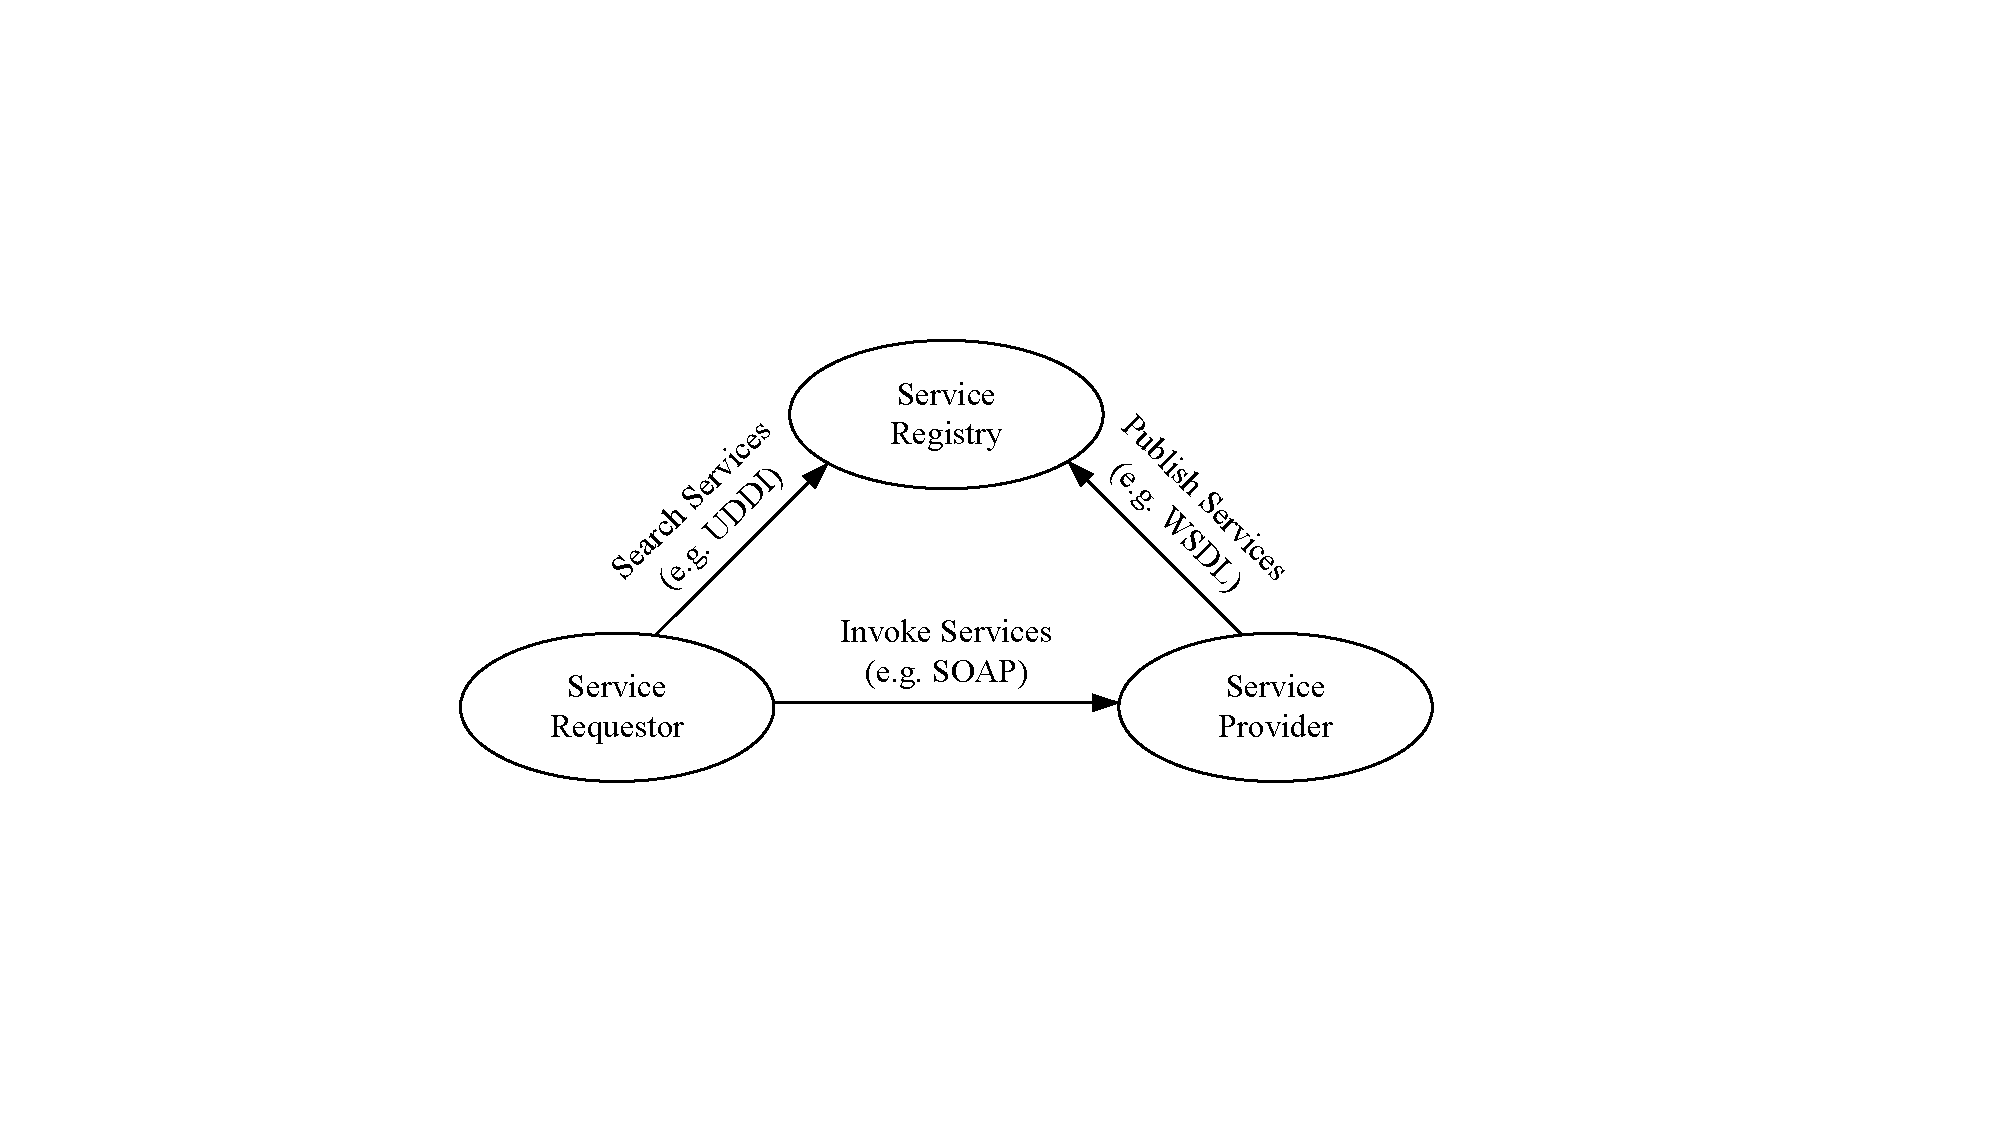
\includegraphics[width=0.5\textwidth]{SOA三角操作模型.pdf}
    \vspace{-1em}
\end{figure}

\begin{spacing}{1.2}
    \vspace{-0.5em}
    \begin{longtable}{|m{7.5cm}|m{7.5cm}|}
        \hline
        \multicolumn{1}{|c|}{\textbf{三种角色}} & \multicolumn{1}{c|}{\textbf{三个操作}} \\ \hline
        \vspace{-1.3em}
        \begin{itemize}[leftmargin=1.5em,itemsep=-3pt]
            \item 服务提供者:发布自己的服务,并且对服务请求进行响应
            \item 服务请求者:利用服务注册查找所需要的服务,然后使用该服务
            \item 服务注册商:注册已经发布的服务,对其进行分类,并提供搜索服务 
        \vspace{-1.5em}
        \end{itemize}                                           
            & 
        \vspace{-1.3em}
        \begin{itemize}[leftmargin=1.5em,itemsep=-3pt]
            \item 发布:为了使服务可访问,需要发布服务描述以使服务使用者可以发现它
            \item 查找:服务请求者查询服务注册来找到满足其标准的服务
            \item 绑定:检索到服务描述后,服务使用者继续根据服务描述中的信息调用服务
        \vspace{-1.5em}
        \end{itemize}  
        \\ \hline
    \end{longtable}
    \vspace{-1em}
\end{spacing}

SOA的优点:
\begin{spacing}{1.2}
    \vspace{-0.5em}
    \begin{longtable}{|m{7.5cm}|m{7.5cm}|}
        \hline
        \multicolumn{1}{|c|}{\textbf{IT优势}} & \multicolumn{1}{c|}{\textbf{商业优势}} \\ \hline
        \vspace{-1.3em}
        \begin{itemize}[leftmargin=1.5em,itemsep=-3pt]
            \item 松耦合,消除假依赖(复用):语言、平台和厂商中立;消除时间依赖;消除访问地址依赖;消除访问协议依赖
            \item 服务间接寻址(灵活)
        \vspace{-1.5em}
        \end{itemize}                                           
            & 
        \vspace{-1.3em}
        \begin{itemize}[leftmargin=1.5em,itemsep=-3pt]
            \item 保护企业投资,提升现有IT资源的作用,促进IT资源的复用
            \item 提高企业灵敏度
            \item 支持企业外包管理模式
        \vspace{-1.5em}
        \end{itemize}  
        \\ \hline
    \end{longtable}
    \vspace{-1em}
\end{spacing}

\end{solution}
	\begin{problem}
XML的结构是什么?与原先的文本/json/二进制相比有什么好处?
\end{problem}

\begin{solution}
XML是一种用于描述数据的标记语言,形成的是树状结构,一个XML文档有唯一的element作为根元素,该元素是所有其他元素的父元素,同时所有的元素均可拥有子元素。XML中的元素由一个开始标签、一个结束标签和其中包含的内容组成。开始标签和结束标签之间的内容可以包含其他元素、文本和属性。

相比于文本、JSON和二进制格式,XML有以下几个优点:
\begin{enumerate}[label=\arabic*.]
    \item 可读性:XML的标记结构和层次关系非常清晰,易于理解和阅读,尤其是对于人类来说。这使得XML非常适合用于传输和存储结构化数据。
    \item XML文档的内容和结构完全分离,基于这个特性可以实现服务的功能管理和流程管理彻底分离。
    \item 互操作性:纯文本文件可以方便地在不同的系统之间通信。
    \item 跨平台性:XML是一种独立于平台和语言的标记语言,可以在不同的操作系统、编程语言和应用程序之间进行交互和传输。
    \item 可扩展性:XML是一种可扩展的标记语言,可以根据需要自定义标记和元素,以适应各种数据结构的需求。
    \item 支持多语言:XML可以支持多种语言和字符集,包括Unicode和其他字符编码,方便多语言系统对数据进行处理。
\end{enumerate}

\end{solution}
	\begin{problem}
试描述SOAP包的结构,并结合该结构,阐述SOAP处理模型(无需准确给出相关命名空间和元素名称)
\end{problem}

\begin{solution}
\begin{figure}[H]
    \vspace{-0.5em}
	\centering
	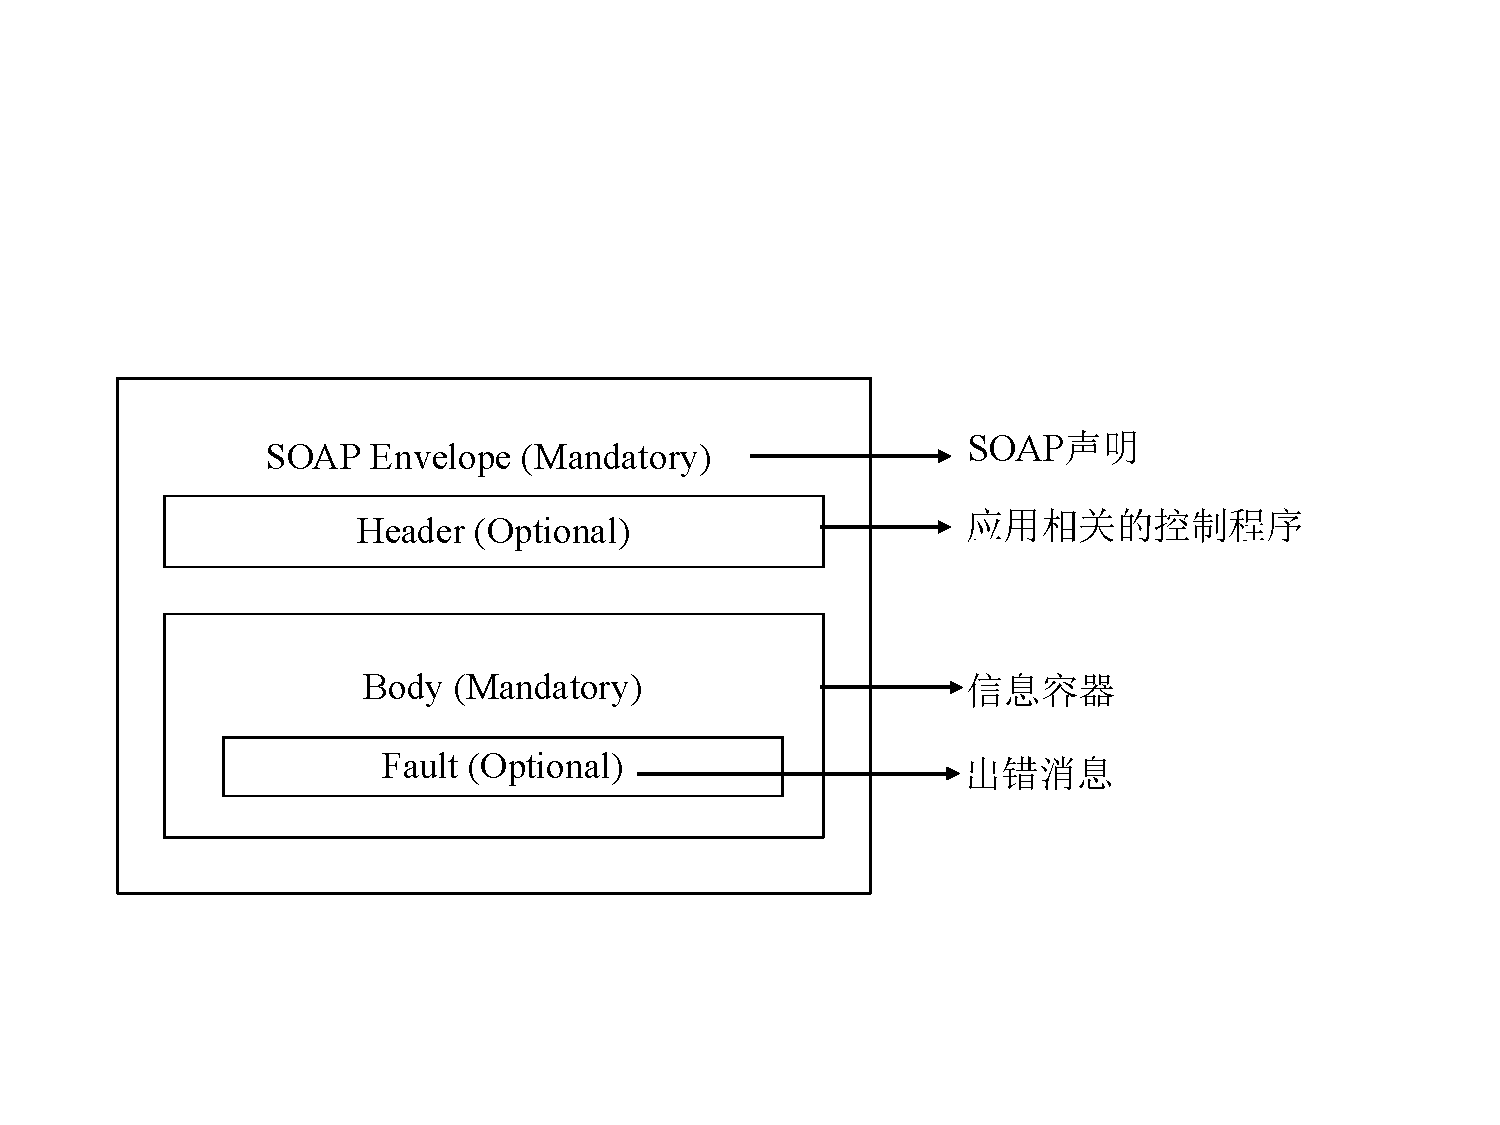
\includegraphics[width=0.65\textwidth]{SOAP结构.pdf}
    \vspace{-1em}
\end{figure}

SOAP包本质是一个XML文档,包含下列元素:
\begin{itemize}
    \item Envelope元素:必需元素,根元素,标识此XML文档为一条 SOAP 消息。可以包含命名空间和声明额外的属性。如果出现额外属性,则必须使用命名空间修饰。
    \item Header 元素:可选元素,有关 SOAP 消息的应用程序专用信息(比如认证、支付等)。
    \item Body 元素:必需元素,包含所有的调用和响应信息。
    \item Fault 元素:可选元素,提供有关在处理此消息所发生错误的信息。
\end{itemize}

SOAP处理模型:
\begin{enumerate}[label=\arabic*.]
    \item 组装SOAP消息:发送方将要发送的数据按照SOAP消息格式进行组装。SOAP消息包括可选的Header和必需的body。
    \item 封装SOAP消息:发送方将组装好的SOAP消息封装成一个标准的HTTP POST请求,然后发送给接收方。封装时需要将SOAP消息体作为HTTP POST请求的请求体(RequestBody)来发送。
    \item 解析SOAP消息:接收方接收到HTTP POST请求后,将请求体中的SOAP消息体进行解析,并提取出其中的数据。
    \item 处理SOAP消息:接收方根据解析出的数据进行业务处理,然后将处理结果封装成SOAP消息格式,通过HTTP响应将处理结果发送回去。
\end{enumerate}

SOAP的两种使用方式:
\begin{figure}[H]
	\setcounter{subfigure}{0}
	\centering
	\vspace{-2em}	
	\subfloat[没有中间转发节点]{
	\begin{minipage}[t]{0.3\linewidth}
	\centering
	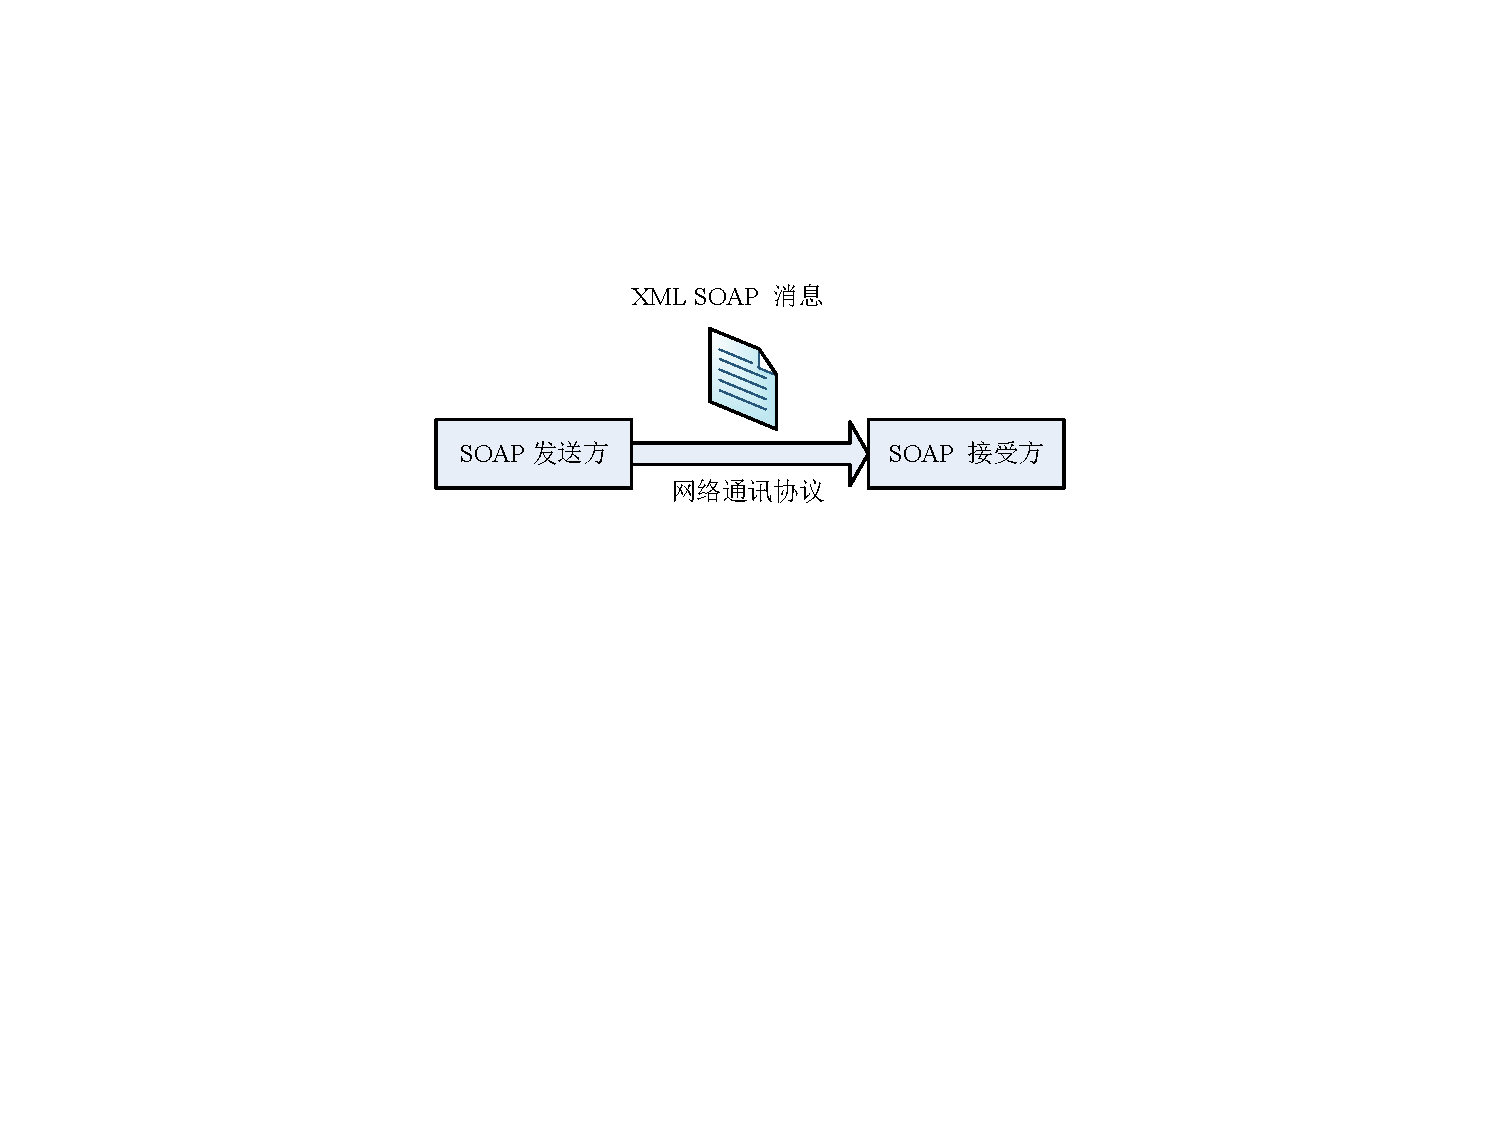
\includegraphics[width=0.97\linewidth]{SOAP没有中间转发节点.pdf}
	\end{minipage}
	}
    \subfloat[有多个中间转发节点]{
	\begin{minipage}[t]{0.66\linewidth}
	\centering
	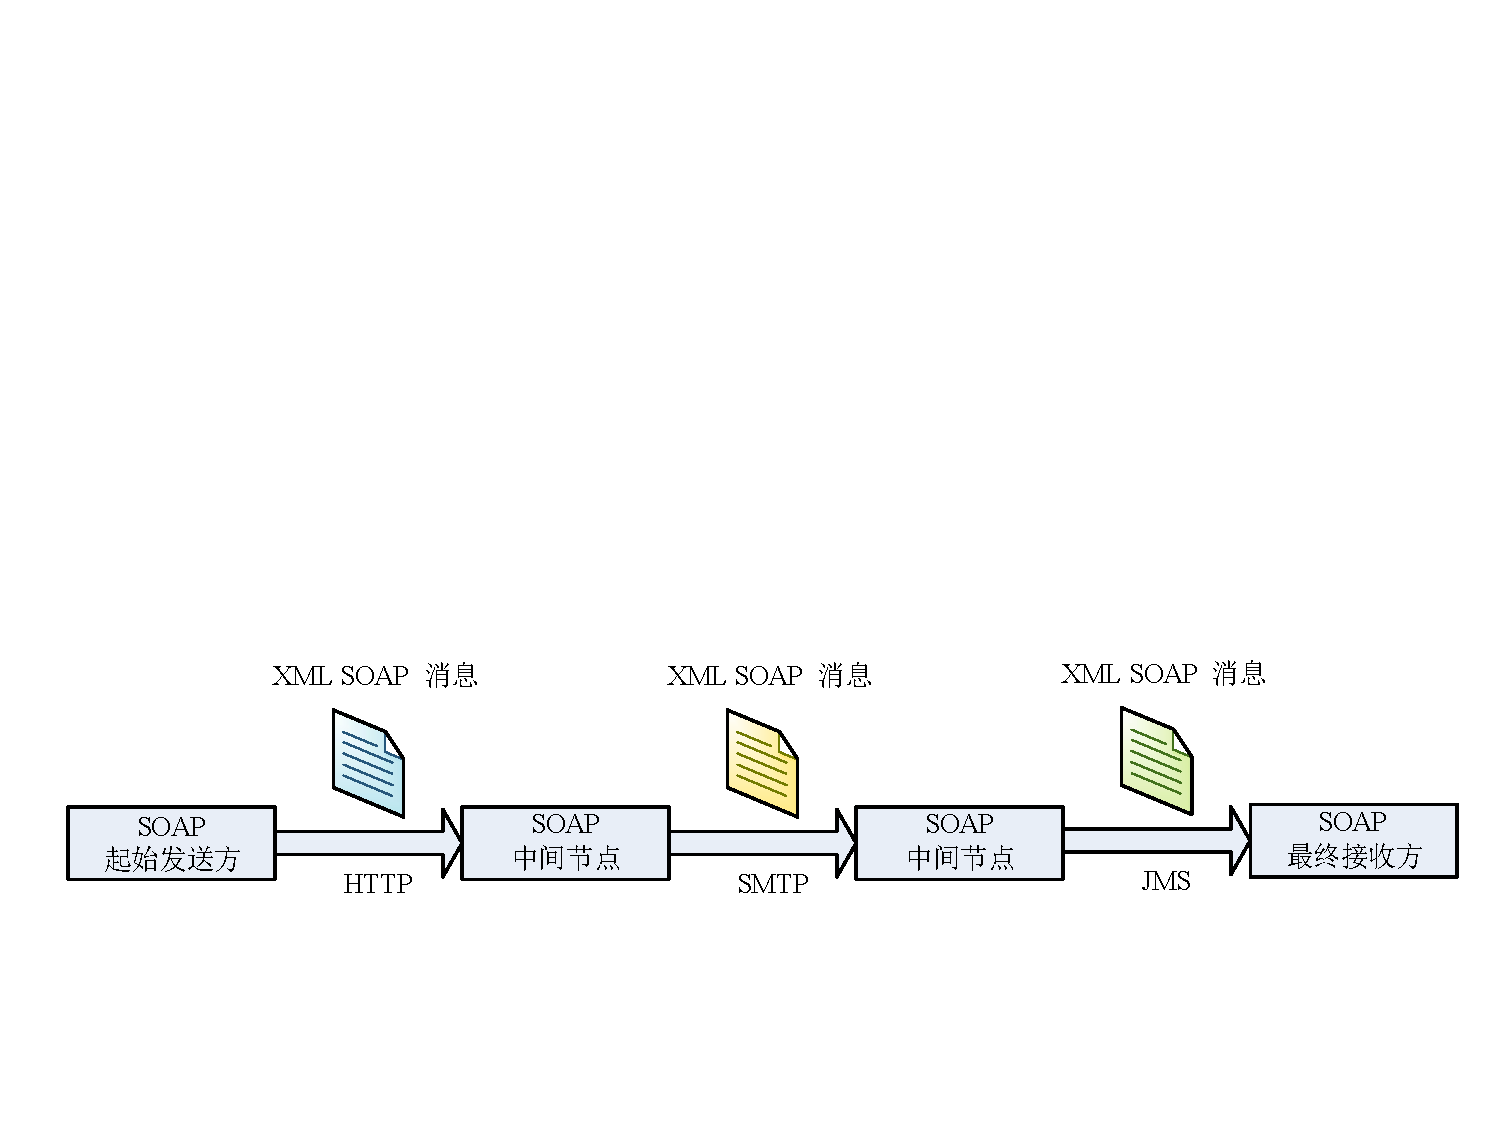
\includegraphics[width=0.93\linewidth]{SOAP有多个中间转发节点.pdf}
	\end{minipage}
	}
	\centering
	\vspace{-1.5em}
\end{figure}

SOAP的两种交互模式:
\begin{spacing}{1.2}
    \vspace{-0.5em}
    \begin{longtable}{|m{7.5cm}|m{7.5cm}|}
        \hline
        \multicolumn{1}{|c|}{\textbf{RPC(远程过程调用)模式}} & \multicolumn{1}{c|}{\textbf{面向文档模式(大多数情况)}} \\ \hline
        \vspace{-1.3em}
        \begin{itemize}[leftmargin=1.5em,itemsep=-3pt]
            \item 同步的请求/应答交互模式
            \item 发送请求并等待响应
        \vspace{-1.5em}
        \end{itemize}                                           
            & 
        \vspace{-1.3em}
        \begin{itemize}[leftmargin=1.5em,itemsep=-3pt]
            \item 异步交互模式
            \item 发送复杂的XML文档,并等待通知,结果会在处理后发回
        \vspace{-1.5em}
        \end{itemize}  
        \\ \hline
    \end{longtable}
    \vspace{-1em}
\end{spacing}

\end{solution}
	\begin{problem}
SOAP为什么被设计成两块?实际SOAP如何利用这两个信道?
\end{problem}

\begin{solution}
SOAP被设计成具有Header和Body两个部分,一方面分离了控制信息和主要数据,让信息结构更更加清晰,在消息传递过程中能够提供更加灵活和可扩展的功能;另一方面,在复杂模式中,header中的头块信息可以和中间节点进行角色上的转变。

SOAP头可以包含一些元素,用于描述SOAP消息的上下文、安全性、事务性等特性,从而更加精细地控制SOAP消息的处理。SOAP头还可以包含自定义的元素,以扩展SOAP消息的功能,比如增加附加信息或调用其他服务。SOAP体包含具体的请求或响应数据,用于传递业务数据。SOAP体可以包含任何类型的XML元素,从而支持复杂的数据结构和业务逻辑。

在实际应用中,SOAP头和SOAP体可以利用不同的信道进行传输,以实现更加灵活和高效的通信。比如,SOAP头可以使用HTTP头部进行传输,SOAP体则可以使用HTTP请求体进行传输。这种方式可以优化SOAP消息的传输效率,同时还可以保证SOAP头和SOAP体的一致性和完整性。

另外,SOAP头和SOAP体也可以利用同一信道进行传输,这种方式可以简化消息传输,但是可能会影响消息的灵活性和可扩展性。
\end{solution}
	\begin{problem}
试结合WSDL文件的结构,说明WSDL文档记载了哪些服务的哪些信息,并阐述为何需要将WSDL文件分为抽象部分和具体部分。
\end{problem}

\begin{solution}
\begin{figure}[H]
    \vspace{-0.5em}
	\centering
	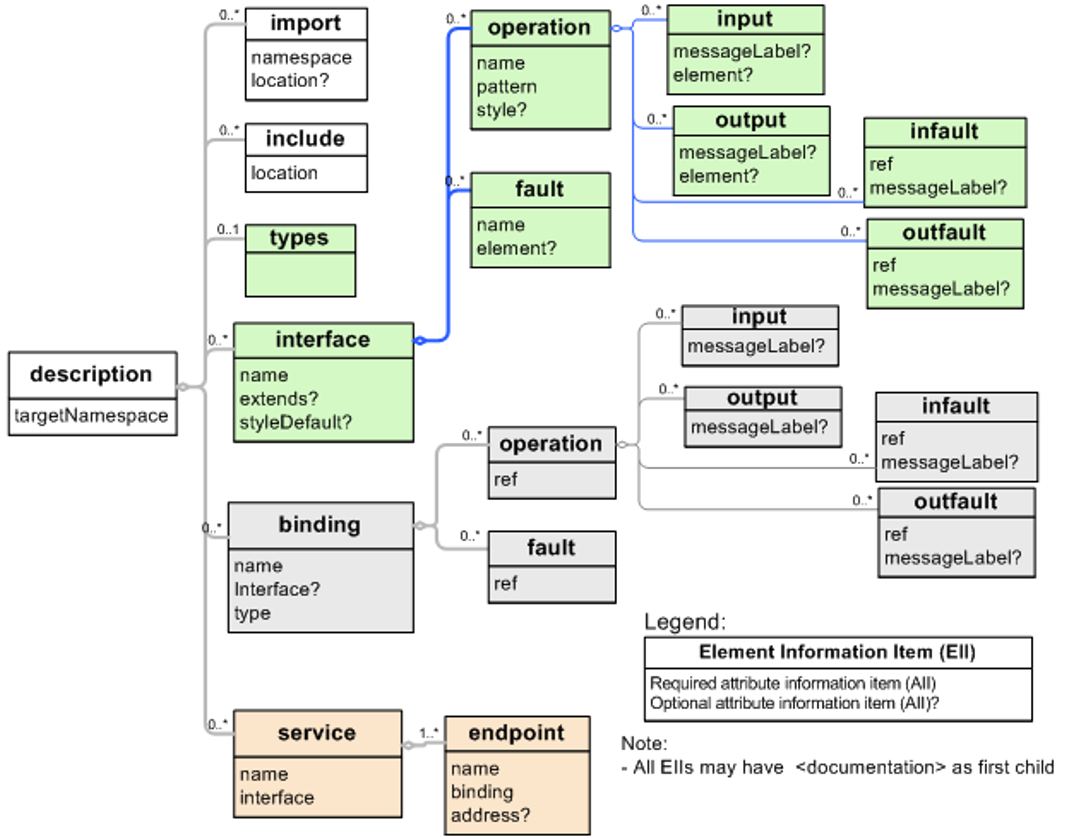
\includegraphics[width=0.68\textwidth]{WSDL 2.0信息集结构.png}
    \vspace{-1em}
\end{figure}

\vspace{-0.5em}
\begin{spacing}{1.2}
    \begin{longtable}{|m{4cm}|m{9cm}|}
        \hline
        \multicolumn{1}{|c|}{WSDL回答了}  &  \multicolumn{1}{c|}{WSDL提供了}\\ \hline
        \vspace{-1.3em}
        \begin{itemize}[leftmargin=1.5em,itemsep=-2pt]
            \item 服务用来干什么
            \item 服务在哪
            \item 如何调用服务
            \vspace{-1.5em}
        \end{itemize} &  
        \vspace{-1.3em}
        \begin{itemize}[leftmargin=1.5em,itemsep=-2pt]
            \item 功能信息(调用某一个特定的操作,这个操作能被用来完成面向服务的一项功能)
            \item 消息结构(如何说明消息交互中的数据类型)
            \item 协议绑定(如何将抽象消息映射为具体的网络传输)
            \vspace{-1.5em}
        \end{itemize}
        \\\hline
    \end{longtable}
\end{spacing}
\vspace{-1em}

\begin{spacing}{1.2}
    \begin{longtable}{|m{8.5cm}|m{6.5cm}|}
        \hline
        \multicolumn{1}{|c|}{\textbf{抽象部分}} & \multicolumn{1}{c|}{\textbf{具体部分}} \\ \hline
        \vspace{-1.3em}
        \begin{itemize}[leftmargin=1.5em,itemsep=-3pt]
            \item Types:独立于机器和语言的类型定义
            \item Message:通信消息的数据结构的抽象类型化定义。使用Types所定义的类型来定义整个消息的数据结构。  
            \item Operation:对服务中所支持的操作的抽象描述,一般单个Operation描述了一个访问入口的请求/响应消息对。
            \item Interface:对于某个访问入口点类型所支持的操作的抽象集合,这些操作可以由一个或多个服务访问点来支持。
        \vspace{-1.5em}
        \end{itemize}                                           
            & 
        \vspace{-1.3em}
        \begin{itemize}[leftmargin=1.5em,itemsep=-3pt]
            \item Binding:特定端口类型的具体协议和数据格式规范的绑定。
            \item Endpoint:定义为协议/数据格式绑定与具体Web访问地址组合的单个服务访问点。
            \item Service:相关服务访问点的集合。
        \vspace{-1.5em}
        \end{itemize}  
        \\ \hline
    \end{longtable}
    \vspace{-1em}
\end{spacing}

WSDL简化结构
\begin{figure}[H]
    \vspace{-0.7em}
	\centering
	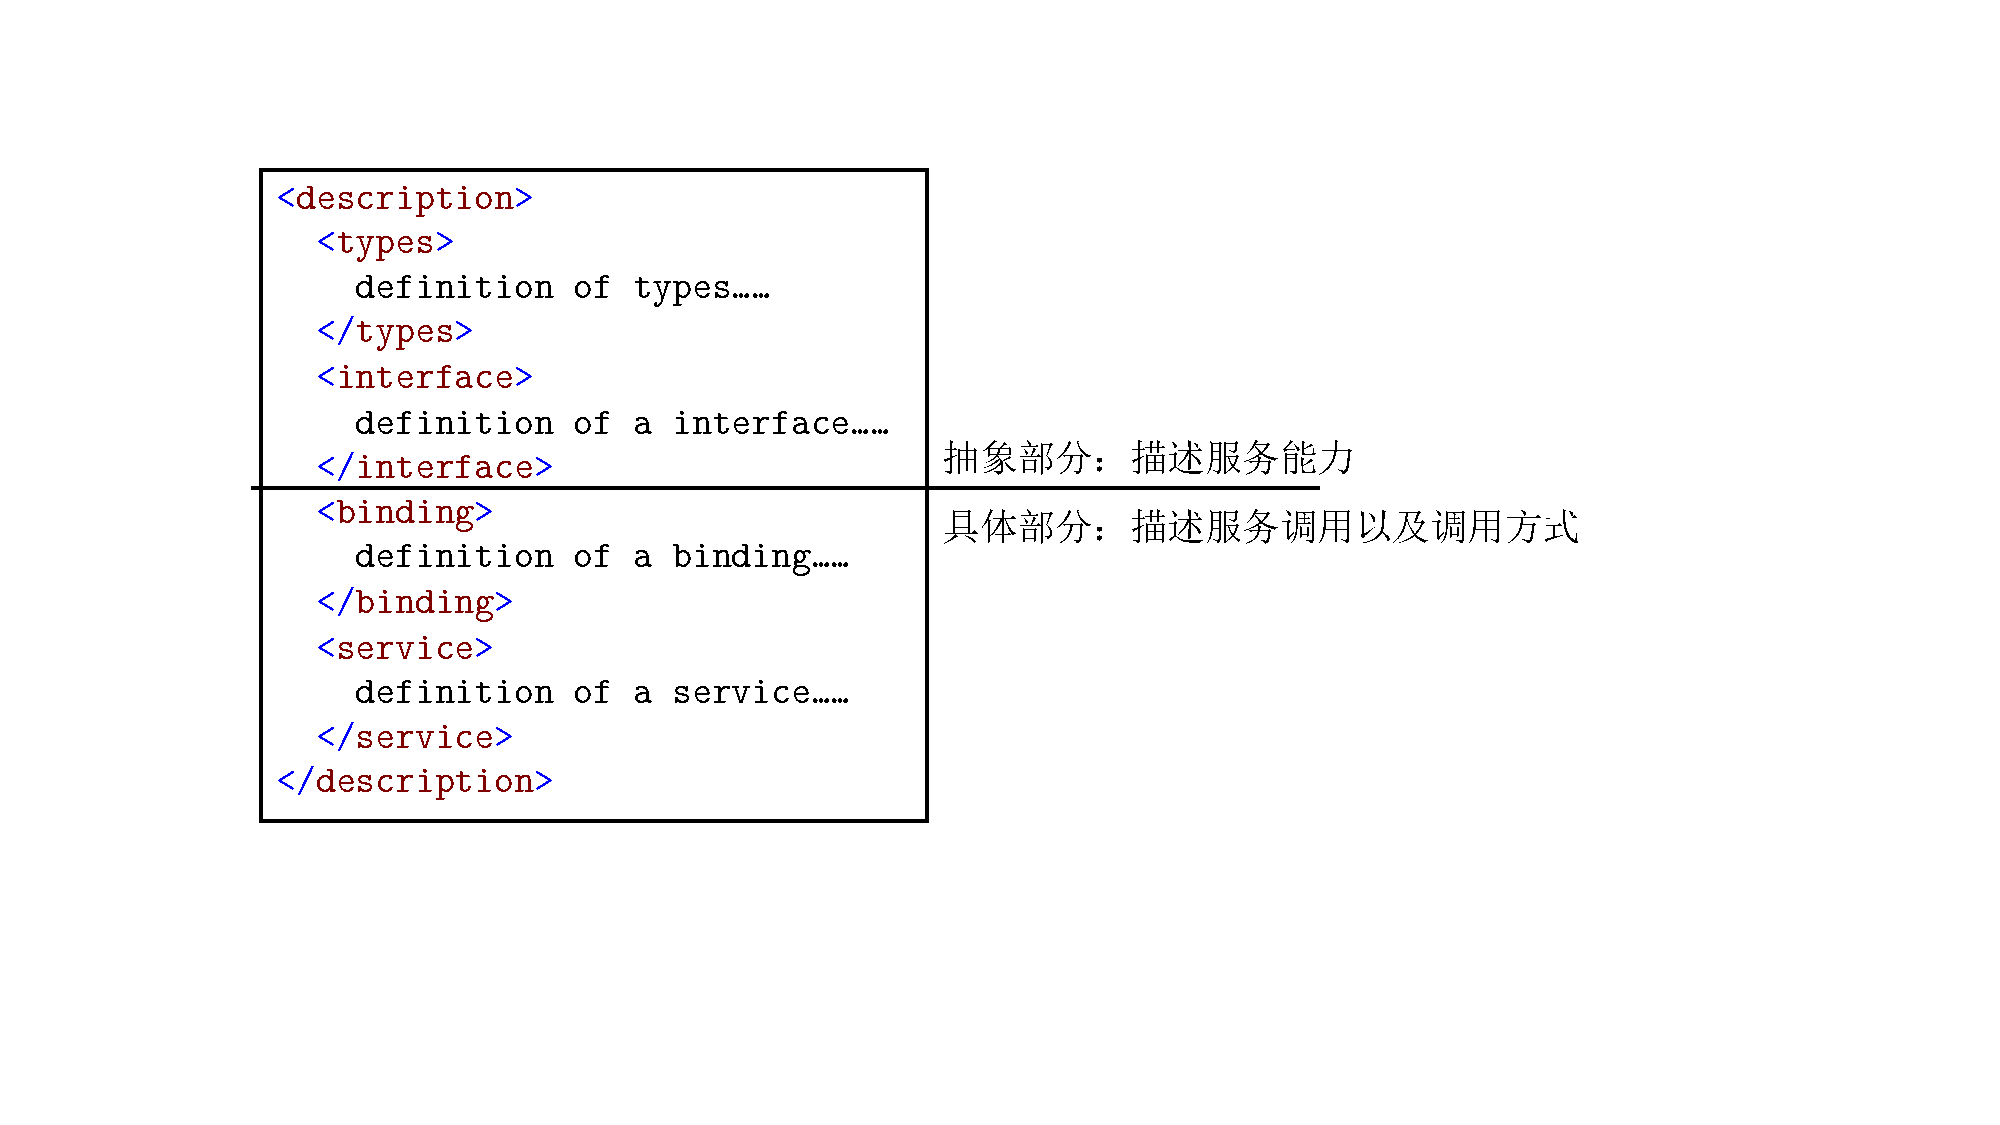
\includegraphics[width=0.7\textwidth]{WSDL简化结构.pdf}
    \vspace{-1em}
\end{figure}

将WSDL文件分为抽象部分和具体部分:
\begin{itemize}
    \item 抽象部分以独立于平台和语言的方式定义服务的逻辑意义,并不包含任何随机器或语言而变的元素,使不同的服务调用者都能调用实现;具体部分则包含了随网站而异的东西,由各实现方依据自己的情况定制。将二者分离能在保证可复用的同时又不局限各实现的个性化定制,同时使得Web服务的接口和实现分离,使得Web服务的接口更加通用和可重用,便于Web服务的维护和扩展,提高互操作性。
    \item 定义服务与实现服务可能是不同的部门或者组织,那么抽象部分与具体部分的WSDL也应当由各自的部门定义、持有与管理。
\end{itemize}

\end{solution}
	\begin{problem}
以UDDI和WSIL为例,分别阐述集中式和分布式服务发布/查询的过程,并对比这两种方法。
\end{problem}

\begin{solution}
\begin{spacing}{1.2}
    \vspace{-0.5em}
    \begin{longtable}{|m{7.5cm}|m{7.5cm}|}
        \hline
        \multicolumn{1}{|c|}{\textbf{集中式发布}} & \multicolumn{1}{c|}{\textbf{集中式查询}} \\ \hline
        \vspace{-1.1em}
        \begin{enumerate}[label=\arabic*.,leftmargin=1.5em,itemsep=-3pt]
            \item 软件公司和标准组织向服务注册发布规范,即tModel
            \item 公司完成服务的开发,注册关于业务及提供的服务的描述
            \item UDDI服务注册给每个实体指定一个唯一的标识符,从而能时刻了解所有实体的情况
        \vspace{-1.3em}
        \end{enumerate}                                           
        & 
        \vspace{-1.1em}
        \begin{enumerate}[label=\arabic*.,leftmargin=1.5em,itemsep=-3pt]
            \item 查询者使用UDDI查询API,根据业务信息、服务信息或服务类别等搜索相关的服务
            \item UDDI找到相应服务的WSDL并生成SOAP发送给查询者,查询者根据WSDL中描述的接口等信息调用服务
        \vspace{-1.3em}
        \end{enumerate}
        \\ \hline
    \end{longtable}
    \vspace{-1em}
    \begin{longtable}{|m{7.5cm}|m{7.5cm}|} 
        \hline
        \multicolumn{1}{|c|}{\textbf{分布式发布}} & \multicolumn{1}{c|}{\textbf{分布式查询}} \\ \hline
        \vspace{-1.1em}
        \begin{enumerate}[label=\arabic*.,leftmargin=1.5em,itemsep=-3pt]
            \item Web服务以XML文档的形式发布到常规 Web 服务器上
            \item 使用WSIL来汇总现有服务描述文档的引用,引用指针可用于连接到在 UDDI 注册表中发布的服务,或连接到另一个 WSIL 文档
            \item 这样不断的连接最终形成WSIL链
        \vspace{-1.3em}
        \end{enumerate}                                           
        & 
        主要基于通过 WSIL 文档链的迭代式搜索过程
        \begin{enumerate}[label=\arabic*.,leftmargin=1.5em,itemsep=-3pt]
            \item 确定起始WSIL文档的位置
            \item 执行指定的WSIL文档搜索
            \item 显示包含在WSIL文档中的链接列表
            \item 选择链接以启动所选WSIL文档的内容。如果所启动的文档包含其他链接,请追踪链接以检索进一步的文档
            \item 重复步骤3和4,迭代所有相关的链接,直到找到所需信息
        \vspace{-1.3em}
        \end{enumerate}  
        \\ \hline
    \end{longtable}
    \vspace{-1em}
\end{spacing}

UDDI和WISL的主要区别在于代价和复杂性:
\begin{itemize}
    \item UDDI适用于希望得到最大复用、得到最大访问范围的服务。 UDDI可以被视为传统的黄页目录,将来自各个组织的已发布 Web 服务进行分类和组织。有着很强的扩展性和可移植性,分门别类,便于管理和共享;但缺点是维护量较大。
    \item WSIL 使得 Web 服务能够通过普通 Web 服务器进行发现、部署和调用,而无需完整而复杂的服务 注册表基础设施。是一个比较便宜用于组织者共享Web服务的解决方案,适用于小型和简单的Web服务。其优点是代价较低。
\end{itemize}

\end{solution}

	\begin{problem}
试结合相关协议和框架,描述一个Web Service从创建开始到被最终服务消费者调用的全过程中对服务的建模、查询和调用(服务生产和服务组合)的全过程。
\end{problem}

\begin{solution}
\begin{figure}[H]
    \vspace{-0.5em}
	\centering
	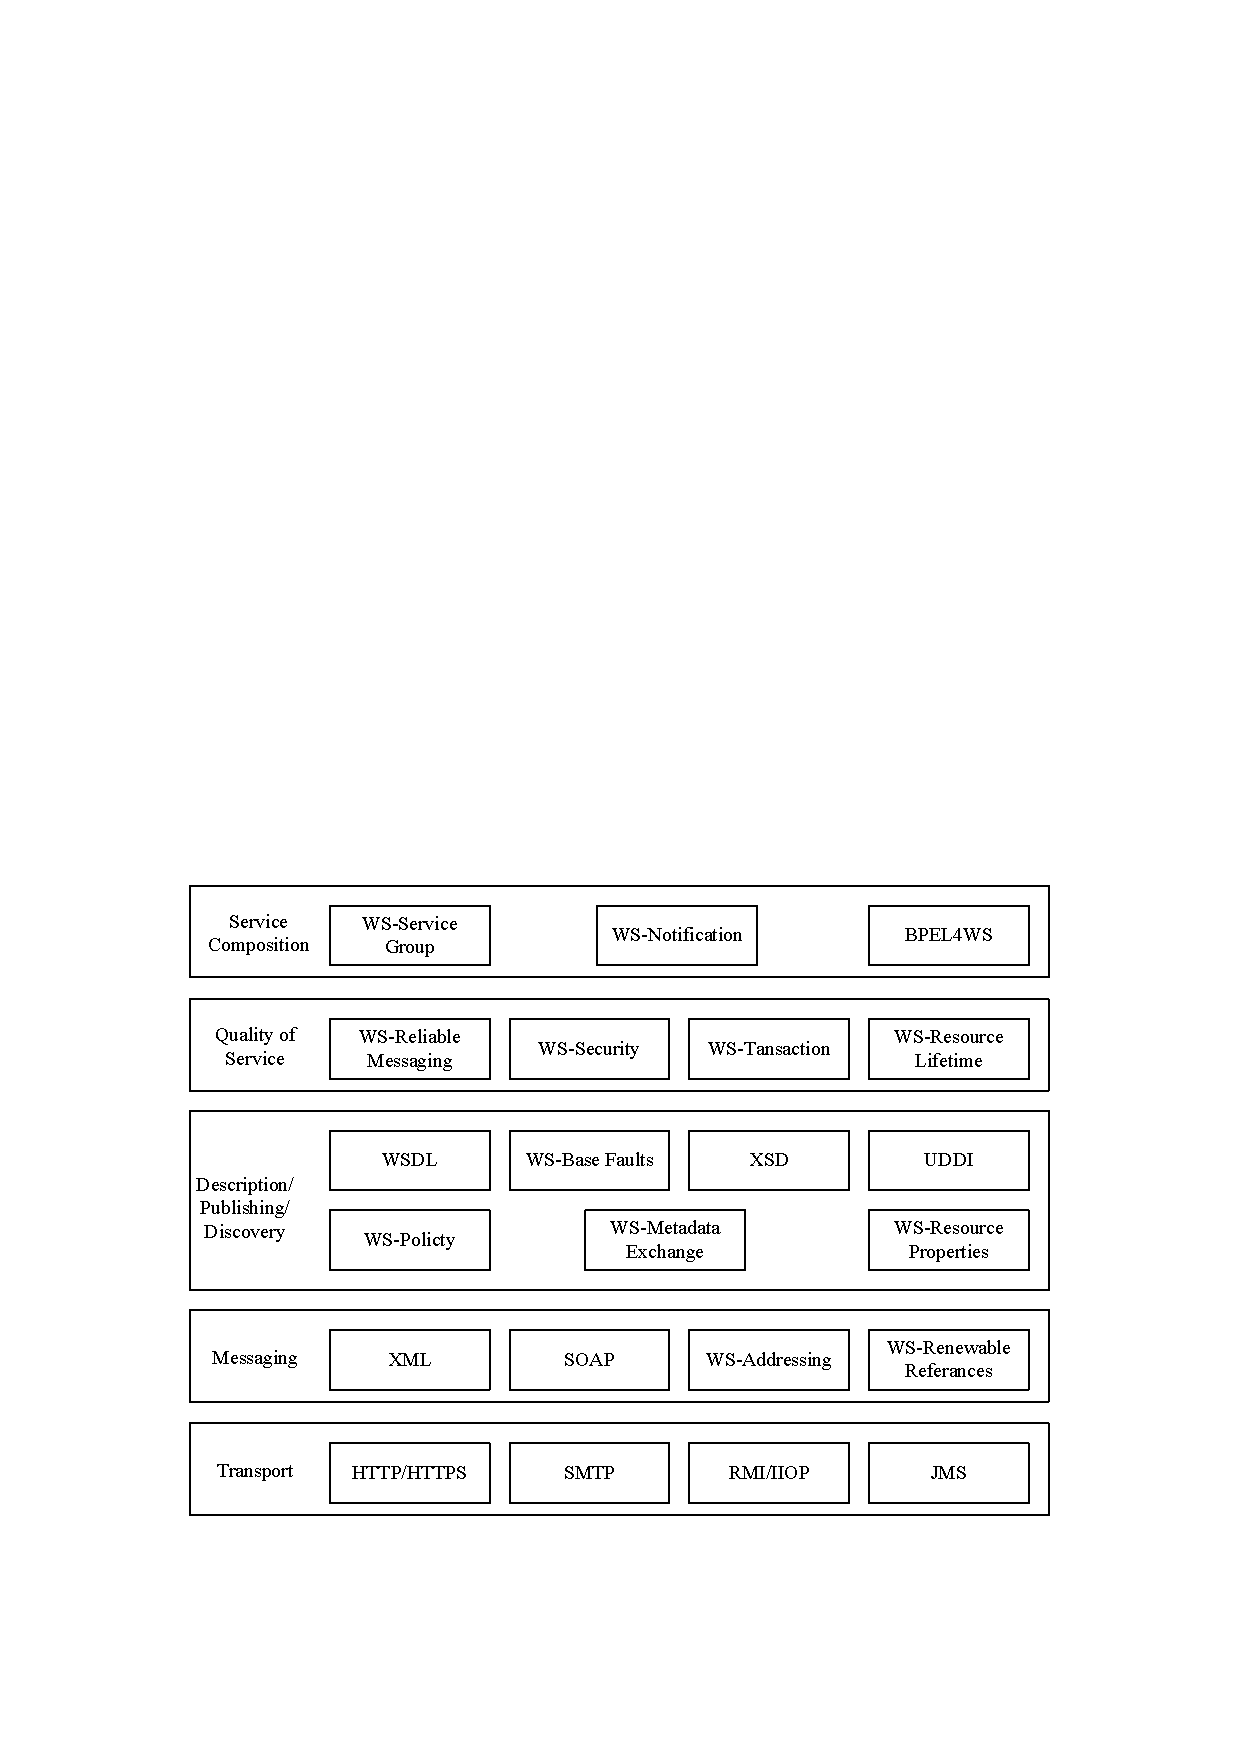
\includegraphics[width=0.75\textwidth]{Web Service过程.pdf}
    \vspace{-1em}
\end{figure}

\textbf{服务的建模}\par
服务建模是Web service 创建的第一步。在此过程中,服务提供者需要确定服务的目标,定义服务的接口和操作,并确定传输协议、消息格式和安全性要求等。在建模过程中,服务提供者可以使用不同的协议和框架,如XML,SOAP,WSDL等。
\begin{itemize}
    \item XML定义了Web服务中的消息交换格式,使用XML Schema定义不同的数据结构,引入Namespace使得XML、XML Schema中的元素和属性全球唯一旦全球共享
    \item SOAP提供了一种标准的方法,使得运行在不同平台、使用不同的技术和编程语言的应用程序可以互相进行通信,服务的发布、查找、调用,都通过SOAP传递XML消息
    \item WSDL对服务能力、服务中使用的数据结构以及传输绑定给出定义和描述;提供了一种基于XML的标准接口定义语言/服务能力定义语言,用以在服务的提供者/调用者/服务注册之间,交换必要的有关Web Service的信息
\end{itemize}

对于大多数服务,使用以上三个协议和框架可以完成建模;对于一些更为复杂的服务,如复合服务或者是带有非功能性需求的服务,还需要用到其他协议和框架完成建模。例如,BPEL定义多个服务间如何交互和合作,从而将一组现有的服务根据业务流程构建起来,实现业务服务。WS-Policy可以实现一些非功能性需求,如信息加密,权限验证等。

\textbf{服务的发布}\par
在此过程中,服务提供者将服务的描述信息发布到注册中心或其它服务目录中,以便服务消费者可以在其中查找并访问到该服务。服务描述信息应包括服务接口、操作、输入输出参数、消息格式、传输协议、安全性要求等信息。该过程可以采用UDDI或WISL方式,其中,UDDI利用分页机制,让服务得到最大可能的复用和共享范围;WSIL使用链连接结构,适用于企业既定的服务。

\textbf{服务的查询(发现)}\par
服务消费者使用服务目录(如UDDI)中的查询功能,以查找并选择适合自己的服务。在查询过程中,服务消费者可以根据服务名称、服务接口、操作、消息格式、传输协议等信息进行筛选和匹配,从而找到符合自己需求的服务。

\textbf{服务的组合}\par
在服务组合阶段,服务消费者可以将多个Web服务组合成一个较为复杂的应用程序。这个过程可以使用BPEL或WS-Coordination协议来实现。BPEL定义了服务组合的业务逻辑,WS-Coordination定义了服务协调和事务处理的规范。

\textbf{服务的调用}\par
在服务调用阶段,服务消费者可以使用客户端代理对象调用远程服务,并使用SOAP消息和XML协议与服务进行通信。服务提供者可以使用WS-Security协议来保护服务的安全性和隐私性。对于可能同时被多个消费者程序使用的服务,WS-Addressing提供了相应的机制,确保服务消费者能在实例池中找到特定的实例并与之通信。对于有状态的服务,可以利用WSRF对状态数据进行存取,进行状态管理,提高资源利用率。

服务调用过程通常包括以下步骤:
\begin{enumerate}[label=\arabic*.]
    \item 构建请求消息:服务消费者根据服务描述信息构建请求消息,并将其发送到服务提供者
    \item 消息传输:请求消息通过网络传输到服务提供者
    \item 消息处理:服务提供者接收到请求消息后,对其进行处理,生成相应消息,并将其发送回服务消费者
    \item 结果处理:服务消费者接收到相应消息后,对其进行处理,获取所需的结果并进行后续处理
\end{enumerate}

\end{solution}
	\begin{problem}
以电信企业为应用背景,举例描述服务分析和服务设计的过程。并结合面向服务的设计原则(标准化服务合约、服务松散耦合、服务抽象、服务可复用性、服务自治、服务无状态性、服务可发现性、服务可组合性),讨论“schema集中化”“合约集中化”“逻辑集中化”在设计过程中的应用。
\end{problem}

\begin{solution}
\textbf{服务分析的过程} \par
面向服务的分析的目标是讨论需要构建哪些服务,每个服务需要封装哪些逻辑
\begin{enumerate}[label=\arabic*.]
    \item 定义流程自动化需求,形成文档化的需求描述,这是服务候选建模的依据
    \item 识别现有的自动化系统,分析企业正在使用的系统具有的功能
    \item 对服务候选建模,识别服务操作候选,并将其分组到服务候选中
\end{enumerate}

在面向服务分析流程中,需要考虑服务可复用性、服务自治和服务可发现性
\begin{itemize}
    \item 可复用性:在服务建模中,需要:精化已有的服务能力候选,使其更加一般化和可复用;定义额外的服务能力候选,这些能力是在构成服务建模过程的基础的业务流程自动化所需之外的
    \item 自治:对已有自动化系统收集得到的信息,会影响服务系统所能达到的自治级别;比如根据信息決定保留遗留系统,那么达到共享自治,独立开发的可能达到逻辑自治或完全自治
    \item 可发现性:从服务生命周期开始,尤其是在产生服务操作候选时,需要以统一的方式,记录所有元数据;在服务建模过程中,业务和技术专家需要一起合作,建立服务候选
\end{itemize}

\textbf{服务设计的过程} \par
服务设计过程,是从服务候选(逻辑)派生出具体的服务设计 (物理),然后装配到实现业务流程的抽象组合中。
\begin{enumerate}[label=\arabic*.]
    \item 组合SOA:选择编排服务层、业务服务层、应用服务层中的哪些进行实现,定义核心的SOA标准,选择SOA扩展(WS-*协议)
    \item 根据业务层级,分别设计以实体为核心的业务服务,应用服务,以任务为核心的业务服务
    \item 设计面向服务业务过程,组合服务构建出业务流程
\end{enumerate}

\textbf{“Schema集中化”} \par
传统的做法是在订购服务、退订服务中使用不同的套餐数据结构,而按照标准化服务合约,所有使用的数据结构都应该被单独定义、管理,与具体的操作流程无关。采用Schema集中化的设计模式,将电信企业划分为多个分离的领域(部门),每个领域都可以被独立地进行标准化和治理,每个领域定义和管理自己的Schema,作为整个服务系统的基本数据结构;在不同的服务中,使用这些Schema,避免了频繁且不必要的数据转换;在必要的情况下,可以利用这些Schema定义新的数据结构。

例如,在电信企业中,可以定义一个名为“用户信息”的Schema, 包括用户ID、姓名、电话号码、地址等信息。然后,各个服务都可以使用这个Schema来定义输入和输出参数,确保它们的数据格式是一致的,这样可以避免数据格式不统一导致的问题。

\textbf{“合约集中化”} \par
为了保证服务松散耦合,避免消极耦合,采用合约集中化,将对服务的访问严格控制在合约内:
\begin{itemize}
    \item 所有的合约应该被集中管理,拥有一致的设计原则和设计目标
    \item 在服务生态系统中,任何情况都不可以绕开合约去访问具体内容
\end{itemize}

合约集中化要求,设计者建立消费者程序时,这些消费者程序仅通过已发布的合约访问一个服务。

为了实现合约集中化,要根据服务抽象、服务可发现性原则设计服务暴露的信息
\begin{itemize}
    \item 服务抽象:技术信息、功能、程序逻辑、服务质量抽象
    \item 服务抽象出来并对外界可用的信息就是服务合约,服务合约的设计标准会影响到又会影响到其他因素
\end{itemize}

例如,在电信企业中,可以定义一个名为“账单查询”的服务合约,其中包括输入参数、输出参数、调用方式和错误处理等信息。各个服务都可以使用这个服务合约来定义自己的接口,确保接口的一致性和兼容性,这样可以避免因为接口不兼容导致的问题。

\textbf{“逻辑集中化”} \par
为了实现服务可复用性,让消费者程序只调用指定的服务,要建立服务库存,在规范的服务库存中,每个服务代表来一个独特的功能域,这就要求服务边界之问没有重叠。

也就是说,当需要某个服务时,首先应该查询服务库存中是否存在已有服务,若有则直接调用;否则应按照面向服务设计原则进行开发并补全到当前服务库存中。

逻辑集中化要求设计者在建立消费者程序并需要特定类型的信息处理时,这些消费者程序只调用指定的服务。

为了实现逻辑集中化,应按照标准化服务合约原则将所有的服务都按照统一的标准进行描述,最大程度的减少调用者无法发现现有服务的可能,进而提高服务的可发现性,从而实现可复用性。服务可发现性是实现服务可复用的前提,服务自治是可复用服务潜在高性能和并行使用的保证;无状态性能提高服务的可用性。

例如,在电信企业中,可以将“账单生成”和“账单发送”两个功能集中在一个名为“账单管理”的服务中实现,然后其他服务可以调用这个服务来生成和发送账单,而不需要每个服务都实现这些功能。这样可以减少代码冗余和维护成本,提高服务的可复用性和可维护性。


为了实现逻辑集中化和合约集中化,Web服务的WSDL、XML schema 和WS-Policy定义必须正确地表达访问一个正式逻辑体(按逻辑集中化)的一个正式访问点(根据合约集中化)。也就是服务消费者调用同一个功能的同一个服务,通过同一个接口来访问后台的实现。
\end{solution}
	\subsubsection*{SOA参考架构}
\begin{figure}[H]
    \vspace{-0.5em}
	\centering
	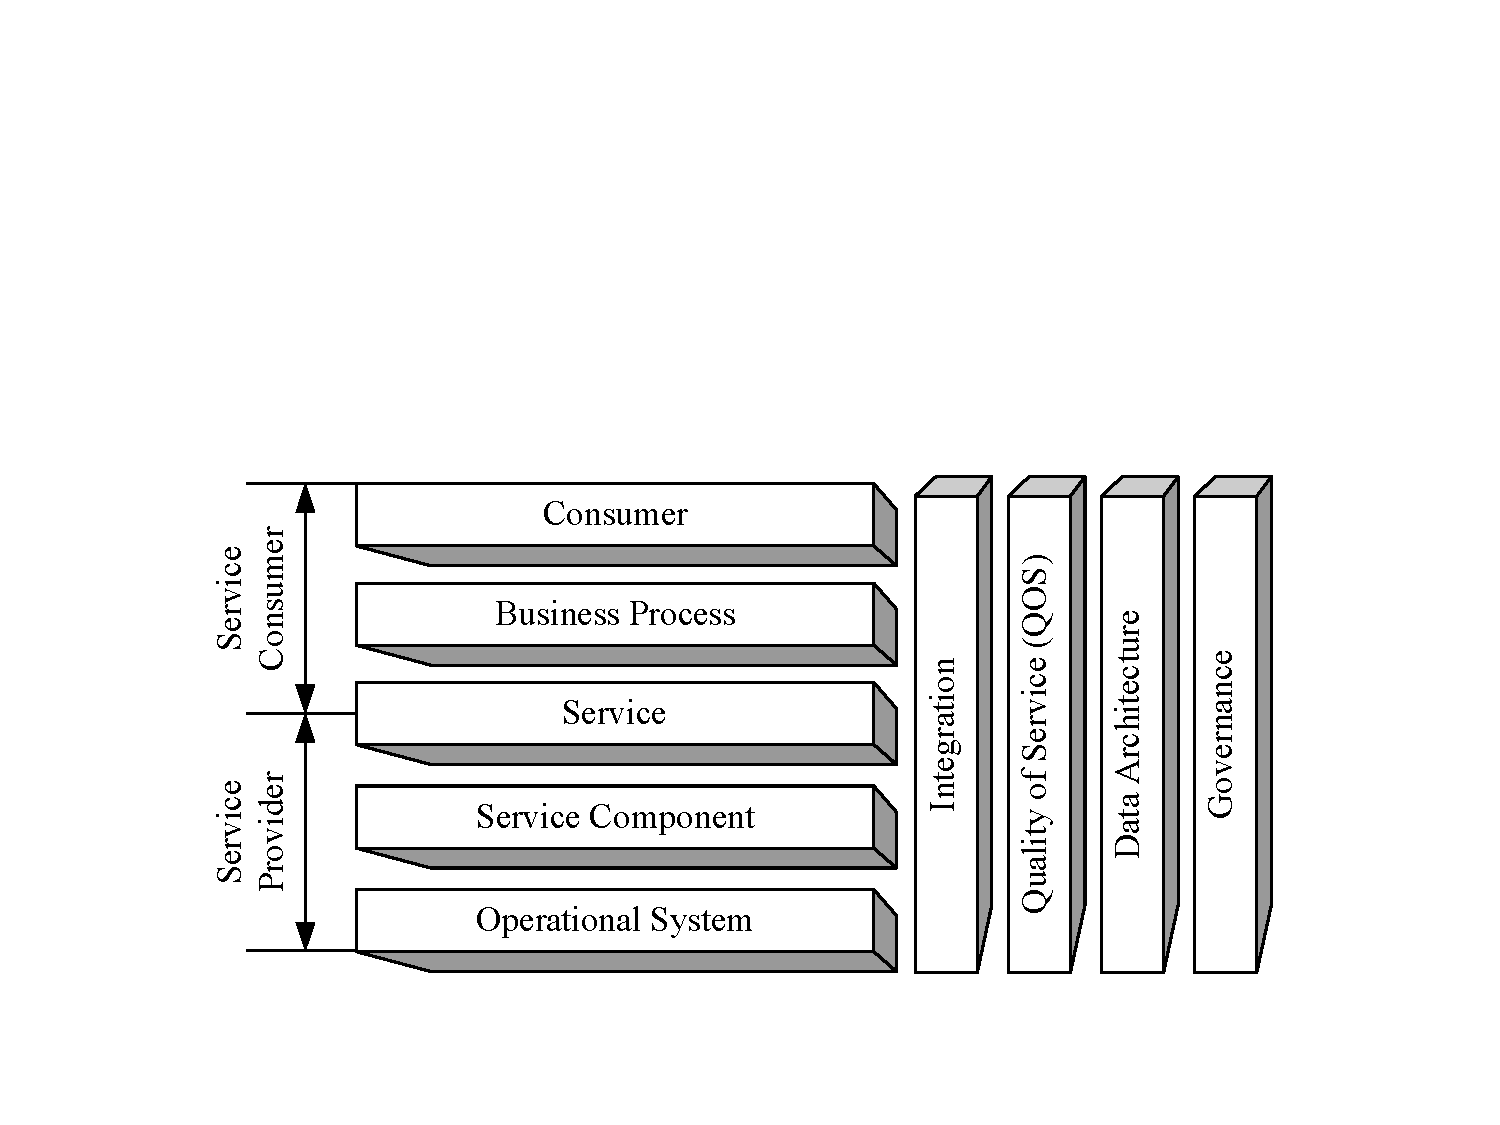
\includegraphics[width=0.7\textwidth]{SOA参考架构.pdf}
    \vspace{-1em}
\end{figure}

水平层:对功能性需求加以满足,五个水平层分为服务提供者和服务消费者两组:
\begin{itemize}
    \item 服务提供者(后台)
\end{itemize}
\begin{spacing}{1.2}
    \begin{table}[H]
    \centering
    \vspace{-0.5em}
    \begin{tabular}{|c|l|}
        \hline
        \textbf{操作型系统层} & \begin{tabular}[c]{@{}l@{}}包括ISV(独立软件开发商)提供的打包应用、客户应用、遗留系统等。\\ 该层的应用(不一定面向服务)往往只为一个目的、服务于一类特定用户。\end{tabular}                                                                                                                                         \\ \hline
        \textbf{服务组件层}  & \begin{tabular}[c]{@{}l@{}}包括用于提供用以实现服务层中所定义服务的代码容器,其中一个服务组件依赖于\\ 操作系统型层次中的一些打包组件、服务层中的一些服务、业务过程层中的一些业\\ 务过程。\\ 该层可能实现多个方法,但其中只有一部分会被服务层封装为服务。\\ 从调用角度出发,服务组件层负责完成输入转换和输出配置的自动化逻辑。\end{tabular}                                                       \\ \hline
        \textbf{服务层}    & \begin{tabular}[c]{@{}l@{}}将SOA三角操作模型扩展为综合的逻辑层次,以支持服务注册、服务分解、服务\\ 发现、服务绑定、接口聚合和生命周期管理。服务层负责定位合适的服务提供者,\\ 并绑定到具体目标服务接口;同时负责以服务组合的形式封装服务对外提供。\\ \textbf{服务簇}是服务层中的核心概念,是一类从概念上服务于同一业务功能的服务集合。\\ 服务簇中的服务可以由不同的功能提供者所发布,并在具体的特性上有所差异(但\\ 都能满足业务功能需求)。\end{tabular} \\ \hline
    \end{tabular}
\end{table}
    \vspace{-2.5em}
\end{spacing}

\begin{itemize}
    \item 服务消费者(前台)
\end{itemize}

\begin{spacing}{1.15}
    \begin{table}[H]
    \centering
    \begin{tabular}{|c|l|}
    \hline
    \textbf{服务层}   & 服务层作为前后台连通的接口,功能同上。   \\ \hline
    \textbf{业务过程层} & \begin{tabular}[c]{@{}l@{}}以组合和分解的方式来处理业务逻辑。\\ 从组合角度出发,业务过程层使用服务层来快速组合服务,并协调业务过程来满足消\\ 费者需求;从分解的角度出发,业务过程层将业务需求分解为能够由概念上的服务簇\\ 所表达的任务。\\ 业务服务层着眼于从协作和管理一些列过程的角度出发,采用也无流程来构建SOA\\解决方案。\\ 存在两种组合方式:编排和编导(二者功能上等价,主流模式为编排)。\end{tabular} \\ \hline
    \textbf{消费者层}  & \begin{tabular}[c]{@{}l@{}}消费者层负责表达对业务过程层、服务层及其他层次的调用。\\ 通过为业务服务快速构建用户接口来满足消费者的需求。\\ 消费者层负责构建SOA解决方案与用户之间进行交互的前端接口。\\ 消费者层可能需要同时支持不同种类的用户和渠道。\\ 为了提升展现性能,往往需要支持缓存机制。\end{tabular}                                                         \\ \hline
    \end{tabular}
\end{table}
    \vspace{-1em}
\end{spacing}

垂直层:对当前系统进行支撑以及实现服务质量、非功能性需求
\begin{spacing}{1.15}
        \begin{table}[H]
        \centering
        \resizebox{\textwidth}{!}{
        \begin{tabular}{|c|l|}
        \hline
        \textbf{集成层}                                                   & \begin{tabular}[c]{@{}l@{}}SOA解决方案中的关键支持部件,用以在服务请求者和服务提供者之间,完成服务请求的 \\ 中介、路由和转换。\end{tabular}                                                 \\ \hline
        \textbf{\begin{tabular}[c]{@{}c@{}}服务质量层\\ (QoS)\end{tabular}} & \begin{tabular}[c]{@{}l@{}}从各个方面(可用性、可靠性、安全性等非功能性需求)提供解决方案层级的QoS管理。\\ 服务质量层不关注于服务层级的QoS控制,而是着眼于为解决方案层级的 QoS 控制提供 \\ 支持、跟踪、监视和管理。\end{tabular} \\ \hline
        \textbf{数据架构层}                                                 & \begin{tabular}[c]{@{}l@{}}为了方便值链集成(集成来源于不同开发方的服务),数据架构层为领域相关的数据架构提 \\ 供统一的表达和支持机制。\end{tabular}                                             \\ \hline
        \textbf{治理层}                                                   & \begin{tabular}[c]{@{}l@{}}提供用以确保 SOA 解决方案的设计原则;通常使用最佳实践的方式,来提供如何在各个层 \\ 次中构建 SOA 解决方案的原则、如何监管运营中的系统,并在运行时处理异常的原则。\end{tabular}               \\ \hline
        \end{tabular}}
    \end{table}
    \vspace{-2em}
\end{spacing}

\begin{itemize}
    \item SOA-RA 展示了如何将 SOA 解决方案构建为一组逻辑层的抽象。
    \item SOA-RA 是一种松耦合的架构,因为每个层不严格隐藏在上面的层之中。
    \item SOA-RA 是一个企业级架构模板,通过定义参考架构指导在企业级别上创建 SOA 解决方案。
    应用 SOA-RA 模型来定义 SOA 导向的系统架构的一种实践称为服务导向建模和架构(SOMA)。
    \item 在SOA-RA层中配置组件定义了三个步骤:
    \vspace{-0.8em}
    \begin{multicols}{3}
    \begin{itemize}
        \item 服务识别步骤
        \item 服务规范步骤
        \item 服务实现步骤
    \end{itemize}
    \end{multicols}
    \vspace{-1em}
\end{itemize}
	\subsubsection*{服务设计原则}

面向服务设计的原则
\vspace{-0.8em}
\begin{multicols}{2}
    \begin{itemize}
        \item \textbf{标准化服务合约:}实现一个标准化合约
        \item \textbf{服务松散耦合:}最小化依赖关系
        \item \textbf{服务抽象:}最小化元信息的可用性
        \item \textbf{服务可复用性:}实现通用的和可复用的逻辑与合约
        \item \textbf{服务自治:}实现独立的功能边界和运行时环境
        \item \textbf{服务无状态性:}实现可适应的,和状态管理无关的逻辑
        \item \textbf{服务可发现性:}实现可交流的元数据
        \item \textbf{服务可组合性:}最大化可组合性
    \end{itemize}
\end{multicols}
\vspace{-1em}

\textbf{标准化服务合约} \par
标准化服务合约与其他原则
\begin{spacing}{1.2}
    \vspace{-0.5em}
    \begin{longtable}{|m{3cm}<{\centering}|m{12cm}|}
    \hline
    标准化服务合约与服务松散耦合
    & 
    \vspace{-1.3em}
    \begin{itemize}[leftmargin=1.5em,itemsep=-3pt,topsep=-3pt]
        \item 消费者和服务之间存在对服务合约中技术接口的依赖
        \begin{itemize}[leftmargin=1.5em,itemsep=-3pt,topsep=-3pt]
            \item 技术服务合约越详细,越内容丰富,消费者和服务之间的依赖关系越强
            \item 两个服务之间所达到的松散耦合程度直接与在服务合约中的依赖关系数量相关
        \end{itemize}
        \item 标准化的合约将会有助于提高服务之间的一致性和耦合质量
    \vspace{-1.5em}
    \end{itemize}  
    \\ \hline
    标准化服务合约与服务抽象 
    & 
    \vspace{-1.3em}
    \begin{itemize}[leftmargin=1.5em,itemsep=-3pt,topsep=-3pt]
        \item 服务抽象原则要求简化合约
        \begin{itemize}[leftmargin=1.5em,itemsep=-3pt,topsep=-3pt]
            \item 非核心信息都被隐藏
        \end{itemize}
        \item 服务合约的设计决定了抽象的程度
        \begin{itemize}[leftmargin=1.5em,itemsep=-3pt,topsep=-3pt]
            \item 在合约中的内容越仔细,服务中被抽象的信息就越少
        \end{itemize}
    \vspace{-1.2em}
    \end{itemize}  
    \\ \hline
    标准化服务合约与服务可复用性 
    & 
    \vspace{-1.3em}
    \begin{itemize}[leftmargin=1.5em,itemsep=-3pt,topsep=-3pt]
        \item 服务可复用性原则常常侧重于服务封装的逻辑是否足够一般和通用
        \item 可复用方案逻辑与数据交换之间的关系最终要由服务合约是如何设计的来决定
        \item 服务合约越是通用、灵活和可扩展,服务的长远复用潜力就越大
    \vspace{-1.5em}
    \end{itemize}  
    \\ \hline
    标准化服务合约与服务可发现性 
    & 
    \vspace{-1.3em}
    \begin{itemize}[leftmargin=1.5em,itemsep=-3pt,topsep=-3pt]
        \item 服务合约越是得到一致的标注和结构化,对于那些需要使用它们的人来说就越是可以预测的
        \item 服务合约越是标准化,元信息的技术接口细节提供得越是充分,服务的可发现性就越高
    \vspace{-1.5em}
    \end{itemize}  
    \\ \hline
    标准化服务合约与服务可组合性 
    & 
    \vspace{-1.3em}
    \begin{itemize}[leftmargin=1.5em,itemsep=-3pt,topsep=-3pt]
        \item 服务的可组合性需求常常与服务合约表达其能力的粒度有关
        \item 粗粒度的操作拥有更高的效率,但常常不适应于需要参与到更大规模组合中的服务
    \vspace{-1.5em}
    \end{itemize}  
    \\ \hline
\end{longtable}
    \vspace{-1em}
\end{spacing}

标准化服务合约设计的风险
\begin{spacing}{1.2}
    \vspace{-0.5em}
    \begin{longtable}{|m{3cm}<{\centering}|m{12cm}|}
    \hline
    版本化(服务合约的演化)
    & 
    \vspace{-1.3em}
    \begin{itemize}[leftmargin=1.5em,itemsep=-3pt,topsep=-3pt]
        \item 服务实施后,就有可能建立起与服务消费者之间的依赖关系
        \item 底层逻辑越是可复用,那些需要消费它的程序的数量和消费频率就会越大
        \item 可扩展性可能引入“破坏”既定合约的重大变化,从而导致发布新的服务版本的要求 
    \vspace{-1.5em}
    \end{itemize}  
    \\ \hline
    技术依赖
    & 
    \vspace{-1.3em}
    \begin{itemize}[leftmargin=1.5em,itemsep=-3pt,topsep=-3pt]
        \item 不同的编程语言和开发平台来实现
        \begin{itemize}[leftmargin=1.5em,itemsep=-3pt,topsep=-3pt]
            \item 使用基于构件的系统并通过增强的RPC技术以支持面向服务
            \item Web Service平台以及它的非专用的通信框架
        \end{itemize} 
        \item 操作性系统层的技术性变化导致服务合约变化
    \vspace{-1.5em}
    \end{itemize}  
    \\ \hline
    开发工具缺陷
    & 
    \vspace{-1.3em}
    \begin{itemize}[leftmargin=1.5em,itemsep=-3pt,topsep=-3pt]
        \item 使用开发工具自动生成合约可能产生非标准化的服务合约
    \vspace{-1.5em}
    \end{itemize}  
    \\ \hline
\end{longtable}
    \vspace{-1em}
\end{spacing}

\textbf{服务松散耦合} \par
服务松散耦合与其他原则
\begin{spacing}{1.2}
    \vspace{-0.5em}
    \begin{longtable}{|m{3cm}<{\centering}|m{12cm}|}
    \hline
    服务松散耦合与标准化服务合约
    & 
    \vspace{-1.3em}
    \begin{itemize}[leftmargin=1.5em,itemsep=-3pt,topsep=-3pt]
        \item 松散耦合鼓励调节技术合约内容的数量和复杂度,从而最小化消费者依赖需求、最大化服务所有者的自由度,在不影响现有消费者的情况下随着时间演化和改变服务
    \vspace{-1.5em}
    \end{itemize}  
    \\ \hline
    服务松散耦合与服务抽象
    & 
    \vspace{-1.3em}
    \begin{itemize}[leftmargin=1.5em,itemsep=-3pt,topsep=-3pt]
        \item 创建更低耦合的消费者关系,明确地要求应用良好定义的功能和技术抽象级别
    \vspace{-1.5em}
    \end{itemize}  
    \\ \hline
    服务松散耦合与服务可复用性
    & 
    \vspace{-1.3em}
    \begin{itemize}[leftmargin=1.5em,itemsep=-3pt,topsep=-3pt]
        \item 减少依赖关系可以使服务更容易被组合、演化甚至扩充以支持不断变化的业务需求和方向
    \vspace{-1.5em}
    \end{itemize}  
    \\ \hline
    服务松散耦合与服务自治
    & 
    \vspace{-1.3em}
    \begin{itemize}[leftmargin=1.5em,itemsep=-3pt,topsep=-3pt]
        \item 减少消极耦合类型的程度,会为运行时和设计时的更高自治级别提供支持
        \item 服务消费者具有越多的跨服务依赖,它所具有的自主权就越少(服务消费者可能同时担任复合服务中的服务协调者)
    \vspace{-1.5em}
    \end{itemize}  
    \\ \hline
    服务松散耦合与服务可发现性
    & 
    \vspace{-1.3em}
    \begin{itemize}[leftmargin=1.5em,itemsep=-3pt,topsep=-3pt]
        \item 服务松散耦合有助于元数据的调节
    \vspace{-1.5em}
    \end{itemize}  
    \\ \hline
    服务松散耦合与服务可组合性
    & 
    \vspace{-1.3em}
    \begin{itemize}[leftmargin=1.5em,itemsep=-3pt,topsep=-3pt]
        \item 在服务组合中,避免消极形式的耦合
        \begin{itemize}[leftmargin=1.5em,itemsep=-3pt,topsep=-3pt]
            \item “合约-逻辑”耦合:如果服务合约是自动生成的,就很有可能在被其他服务使用时不符合标准。因此需要在它和其他组成成员之间进行转换
            \item “合约-技术”耦合:如果同一个组合中的不同部分同时使用开放与专用服务技术,就会需要在本地实现技术转化层
            \item “合约-实现”耦合:当一个服务合约与底层实现特性之间产生耦合时,就会最终把这些性质强加到作为一个整体的组合之上
        \end{itemize} 
    \vspace{-1.2em}
    \end{itemize}  
    \\ \hline
\end{longtable}
    \vspace{-1em}
\end{spacing}

服务松散耦合的相关风险
\begin{spacing}{1.2}
    \vspace{-0.5em}
    \begin{longtable}{|m{3cm}<{\centering}|m{12cm}|}
    \hline
    “逻辑-合约”耦合的限制
    & 
    \vspace{-1.3em}
    \begin{itemize}[leftmargin=1.5em,itemsep=-3pt,topsep=-3pt]
        \item 同一底层逻辑对应两个或者多个合约,从而建立多个入口,每一入口向不同类型的消费者暴露不同的服务能力
    \vspace{-1.5em}
    \end{itemize}  
    \\ \hline
    Schema耦合太“松散”
    & 
    \vspace{-1.3em}
    \begin{itemize}[leftmargin=1.5em,itemsep=-3pt,topsep=-3pt]
        \item 为了强调服务的兼容性演化能力,通过过分简化服务合约,追求减少消费者依赖,仅确定了一些非常通用的数据类型(弱类型)
        \item 验证并处理弱类型,增加服务所需的性能要求
        \item 服务合约发布的信息越少,消费者程序就需要知道越多关于服务实现逻辑的信息,从而产生消极耦合  
    \vspace{-1.5em}
    \end{itemize}  
    \\ \hline
\end{longtable}
    \vspace{-1em}
\end{spacing}

\textbf{服务抽象} \par
服务抽象与其他原则
\begin{spacing}{1.2}
    \vspace{-0.5em}
    \begin{longtable}{|m{3cm}<{\centering}|m{12cm}|}
    \hline
    服务抽象与标准化服务合约
    & 
    \vspace{-1.3em}
    \begin{itemize}[leftmargin=1.5em,itemsep=-3pt,topsep=-3pt]
        \item 服务抽象出来并对外界可用的信息就是服务合约,服务抽象原则的应用影响到服务合约
        \item 服务合约的设计标准也会影响到功能、技术和逻辑抽象的等级 
    \vspace{-1.5em}
    \end{itemize}  
    \\ \hline
    服务抽象与服务松散耦合
    & 
    \vspace{-1.3em}
    \begin{itemize}[leftmargin=1.5em,itemsep=-3pt,topsep=-3pt]
        \item 抽象的程度对可能耦合的程度有直接的关系
        \item 少量的高度详细的技术接口约束会导致比大量含糊或开放的数据约束更多的紧密耦合需求
        \begin{itemize}[leftmargin=1.5em,itemsep=-3pt,topsep=-3pt]
            \item 耦合的程度一般由被抽象的信息数量和信息本身的属性的组合来决定
            \item 最终由服务合约的粒度加以体现 
        \end{itemize}
    \vspace{-1.2em}
    \end{itemize}  
    \\ \hline
    服务抽象与其他原则
    & 
    \vspace{-1.3em}
    \begin{itemize}[leftmargin=1.5em,itemsep=-3pt,topsep=-3pt]
        \item 其他的服务设计原则,如服务可复用性、服务可组合性和服务可发现性等原则都鼓励创建更多的、关于服务的元信息
        \item 而服务的抽象原则要求在发布这些元信息前评估其必要程度
    \vspace{-1.5em}
    \end{itemize}  
    \\ \hline
\end{longtable}
    \vspace{-1em}
\end{spacing}

服务抽象的相关风险
\begin{spacing}{1.2}
    \vspace{-0.5em}
    \begin{longtable}{|m{3cm}<{\centering}|m{12cm}|}
    \hline
    多消费者耦合的需求
    & 
    \vspace{-1.3em}
    \begin{itemize}[leftmargin=1.5em,itemsep=-3pt,topsep=-3pt]
        \item 不同消费者可能需要不同的技术接口细节,所需的抽象程度也不尽相同
        \item 使用合约反规范化,提供不同级别的抽象粒度
    \vspace{-1.5em}
    \end{itemize}  
    \\ \hline
    人为误判
    & 
    \vspace{-1.3em}
    \begin{itemize}[leftmargin=1.5em,itemsep=-3pt,topsep=-3pt]
        \item 过于抽象的服务合约导致曲解或不能充分理解一个服务。从而丧失潜在的复用机会
        \item 过于具体的服务合约导致对服务的行为作出与服务实现相关的假设,从而导致实现耦合
    \vspace{-1.5em}
    \end{itemize}  
    \\ \hline
    安全和隐私的考虑
    & 
    \vspace{-1.3em}
    \begin{itemize}[leftmargin=1.5em,itemsep=-3pt,topsep=-3pt]
        \item 服务合约可能暴露私有或者敏感信息
        \begin{itemize}[leftmargin=1.5em,itemsep=-3pt,topsep=-3pt]
            \item 不同的使用环境(组织内部 vs. 组织外部)
            \item 并发和冗余的服务合约内容以解决这一问题
        \end{itemize}
    \vspace{-1.2em}
    \end{itemize}  
    \\ \hline
\end{longtable}
    \vspace{-1em}
\end{spacing}

\textbf{服务可复用性} \par
服务可复用性与其他原则
\begin{spacing}{1.2}
    \vspace{-0.5em}
    \begin{longtable}{|m{3cm}<{\centering}|m{12cm}|}
    \hline
    服务可复用性与标准化服务合约
    & 
    \vspace{-1.3em}
    \begin{itemize}[leftmargin=1.5em,itemsep=-3pt,topsep=-3pt]
        \item 可复用的服务需要足够的灵活性来支持带有不同交互需求的消费者
        \item 导致降低合约验证约束(尤其是那些易变的)的设计标准
    \vspace{-1.5em}
    \end{itemize}  
    \\ \hline
    服务可复用性与服务抽象
    & 
    \vspace{-1.3em}
    \begin{itemize}[leftmargin=1.5em,itemsep=-3pt,topsep=-3pt]
        \item 合约的自描述性与简洁之间的平衡
        \item 元信息的抽象程度反映这一平衡 
    \vspace{-1.5em}
    \end{itemize}  
    \\ \hline
    服务可复用性与服务松散耦合
    & 
    \vspace{-1.3em}
    \begin{itemize}[leftmargin=1.5em,itemsep=-3pt,topsep=-3pt]
        \item 一个服务的依赖需求越小,复用它就越简单
        \item 当追求服务逻辑的可复用性时,总是有一种减少服务合约约束的趋势
    \vspace{-1.5em}
    \end{itemize}  
    \\ \hline
    服务可复用性与其他原则
    & 
    \vspace{-1.3em}
    \begin{itemize}[leftmargin=1.5em,itemsep=-3pt,topsep=-3pt]
        \item 服务自治:自治是对可复用服务潜在高性能和并行使用的保证
        \item 服务无状态:通过最小化状态管理责任,提高一个服务的可用性,从而提高有效扩展的能力
        \item 服务可发现性:可复用服务必需可发现、可解释
        \item 服务可组合性:可组合是复用的一种形式,可复用潜能越大,服务被反复组装的机会就越大 
    \vspace{-1.5em}
    \end{itemize}  
    \\ \hline
\end{longtable}
    \vspace{-1em}
\end{spacing}

服务可复用性的相关风险
\begin{spacing}{1.2}
    \vspace{-0.5em}
    \begin{longtable}{|m{3cm}<{\centering}|m{12cm}|}
    \hline
    文化上的考虑
    & 
    \vspace{-1.3em}
    \begin{itemize}[leftmargin=1.5em,itemsep=-3pt,topsep=-3pt]
        \item 程序员和架构师不愿意去使用
    \vspace{-1.5em}
    \end{itemize}  
    \\ \hline
    治理上的考虑
    & 
    \vspace{-1.3em}
    \begin{itemize}[leftmargin=1.5em,itemsep=-3pt,topsep=-3pt]
        \item 面向服务将相互无关的逻辑单元抽象为服务,与业务流程、应用程序或用户基础都没有任何直接联系
    \vspace{-1.5em}
    \end{itemize}  
    \\ \hline
    可靠性上的考虑
    & 
    \vspace{-1.3em}
    \begin{itemize}[leftmargin=1.5em,itemsep=-3pt,topsep=-3pt]
        \item 可复用服务的单点失效会导致多个业务流程的失败
        \item 通过对关键服务的多重复用来解决
    \vspace{-1.5em}
    \end{itemize}  
    \\ \hline
    安全上的考虑
    & 
    \vspace{-1.3em}
    \begin{itemize}[leftmargin=1.5em,itemsep=-3pt,topsep=-3pt]
        \item 在不同应用场景中的安全性要求不同
        \item 安全级别可能和信息交换的方式直接相关,甚至可能和服务合约所暴露的功能类型相关
    \vspace{-1.5em}
    \end{itemize}  
    \\ \hline
    商业设计需求上的考虑
    & 
    \vspace{-1.3em}
    \begin{itemize}[leftmargin=1.5em,itemsep=-3pt,topsep=-3pt]
        \item 领域专家在进行服务分析和建模阶段中引入的风险和问题
    \vspace{-1.5em}
    \end{itemize}  
    \\ \hline
    敏捷交付上的考虑
    & 
    \vspace{-1.3em}
    \begin{itemize}[leftmargin=1.5em,itemsep=-3pt,topsep=-3pt]
        \item 在需要以敏捷开发方法来解决短期和战术上的业务目标时,提倡服务的可复用性是非常困难的
    \vspace{-1.5em}
    \end{itemize}  
    \\ \hline
\end{longtable}
    \vspace{-1em}
\end{spacing}

\textbf{服务自治} \par
服务自治与其他原则
\begin{spacing}{1.2}
    \vspace{-0.5em}
    \begin{longtable}{|m{3cm}<{\centering}|m{12cm}|}
    \hline
    服务自治与标准化服务合约
    & 
    \vspace{-1.3em}
    \begin{itemize}[leftmargin=1.5em,itemsep=-3pt,topsep=-3pt]
        \item 服务合约自治直接与服务合约紧密相连
        \item 规范化的考虑会影响到合约如何形成,以及如何与其他服务协调
        \item 在服务合约上有越大的控制权,服务合约能被更好地定制和标准化,越能够确保底层实现可以在遵循既定自治级别的前提下,被独立设计
    \vspace{-1.5em}
    \end{itemize}  
    \\ \hline
    服务自治与服务松散耦合
    & 
    \vspace{-1.3em}
    \begin{itemize}[leftmargin=1.5em,itemsep=-3pt,topsep=-3pt]
        \item 由于同样期望将服务之间的依赖最小化,服务自治在很大程度上支持服务松散耦合原则:积极耦合会直接导致设计时自治的增加;设计时自治的增加,又能更好地增强和优化服务的实现,从而支持运行时的自治
    \vspace{-1.5em}
    \end{itemize}  
    \\ \hline
    服务自治与服务抽象
    & 
    \vspace{-1.3em}
    \begin{itemize}[leftmargin=1.5em,itemsep=-3pt,topsep=-3pt]
        \item 将一个服务的自治级别作为整个服务合约的一部分来发布
        \item 服务自治的信息是服务质量信息抽象的一个例子
    \vspace{-1.5em}
    \end{itemize}  
    \\ \hline
    服务自治与服务可复用性
    & 
    \vspace{-1.3em}
    \begin{itemize}[leftmargin=1.5em,itemsep=-3pt,topsep=-3pt]
        \item 自治的增加提高了一个服务的复用潜力
        \item 通过增强服务的可靠性和提高服务行为的可预测性,其逻辑可以更加容易地适应多个服务消费者的需求
        \item 更好地支持服务运行环境的演化,从而应对复用所带来的并发要求 
    \vspace{-1.5em}
    \end{itemize}  
    \\ \hline
    服务自治与服务无状态性
    & 
    \vspace{-1.3em}
    \begin{itemize}[leftmargin=1.5em,itemsep=-3pt,topsep=-3pt]
        \item 实现高级别的服务自治可以直接支持服务无状态性程度的增加
    \vspace{-1.5em}
    \end{itemize}  
    \\ \hline
    服务自治与服务可组合性
    & 
    \vspace{-1.3em}
    \begin{itemize}[leftmargin=1.5em,itemsep=-3pt,topsep=-3pt]
        \item 服务组合的整体自治性取决于它的所有组成成员自身的自治性
        \item 服务有越好的可靠性和可预侧性就越能组成更高效的大型服务组合 
    \vspace{-1.5em}
    \end{itemize}  
    \\ \hline
\end{longtable}
    \vspace{-1em}
\end{spacing}

服务自治的相关风险
\begin{spacing}{1.2}
    \vspace{-0.5em}
    \begin{longtable}{|m{3cm}<{\centering}|m{12cm}|}
    \hline
    错误地判断服务的范围
    & 
    \vspace{-1.3em}
    \begin{itemize}[leftmargin=1.5em,itemsep=-3pt,topsep=-3pt]
        \item 服务自治倾向于产生隔离的服务
        \item 如果在服务建模过程中,错误计算或者错误判断了服务的范围定义,在被部署到一个隔离的环境之后,将很难再被改变
        \item 服务能力也有类似的问题
    \vspace{-1.5em}
    \end{itemize}  
    \\ \hline
    包装服务和遗留逻辑封装
    & 
    \vspace{-1.3em}
    \begin{itemize}[leftmargin=1.5em,itemsep=-3pt,topsep=-3pt]
        \item 与封装相关联的服务自治风险包括:
        \begin{itemize}[leftmargin=1.5em,itemsep=-3pt,topsep=-3pt]
            \item 为了实现服务而使用的服务适配器不够灵活,并且无法被充分定制。这会威胁到标准化和可发现性这类设计特性
            \item 底层遗留环境是无法被定制的,因而会危害到其他面向服务原则的应用
        \end{itemize} 
        \item 当服务的实现需要封装遗留逻辑时,它所能达到的自治级别几乎总是会明显降低
    \vspace{-1.5em}
    \end{itemize}  
    \\ \hline
    对服务需求的过高估计
    & 
    \vspace{-1.3em}
    \begin{itemize}[leftmargin=1.5em,itemsep=-3pt,topsep=-3pt]
        \item 服务自治要求较高的资源,长期高估服务的使用需求,可能会在一定程度上破坏面向服务计算的减低IT负载的目标
        \item 因此,即使资源非常充裕,对需要达到较高自治级别的服务也需逐个进行代价评估
    \vspace{-1.5em}
    \end{itemize}  
    \\ \hline
\end{longtable}
    \vspace{-1em}
\end{spacing}

\textbf{服务无状态性} \par
服务无状态性与其他原则
\begin{spacing}{1.2}
    \vspace{-0.5em}
    \begin{longtable}{|m{3cm}<{\centering}|m{12cm}|}
    \hline
    服务无状态性与服务可复用性
    & 
    \vspace{-1.3em}
    \begin{itemize}[leftmargin=1.5em,itemsep=-3pt,topsep=-3pt]
        \item 减少活动相关逻辑使一个服务变得更加无关(而无关服务具有更好的可复用性)
        \item 提高服务的可扩展性和可用性使得它们可以在更多的服务组合中被更多的服务消费者复用
    \vspace{-1.5em}
    \end{itemize}  
    \\ \hline
    服务无状态性与服务自治
    & 
    \vspace{-1.3em}
    \begin{itemize}[leftmargin=1.5em,itemsep=-3pt,topsep=-3pt]
        \item 状态信息的本质通常是特定于一个给定的活动或者业务流程的,通过在服务边界外改变状态管理机制和流程的职责,就可以降低服务逻辑依赖于更大的业务任务的可能性。这使得服务能够更加自给自足,并且能够被定位成技术环境的一个独立部分,因而直接增加其整体自治性
        \item 另一方面,由环境架构所提供的状态管理延迟选项可要求服务形成在其边界外的一个直接依赖。这种类型的外部实现耦合会影响到一个服务的整体自治
    \vspace{-1.5em}
    \end{itemize}  
    \\ \hline
\end{longtable}

    \vspace{-1em}
\end{spacing}

服务无状态性的相关风险
\begin{spacing}{1.2}
    \vspace{-0.5em}
    \begin{longtable}{|m{3cm}<{\centering}|m{12cm}|}
    \hline
    对于架构的依赖
    & 
    \vspace{-1.3em}
    \begin{itemize}[leftmargin=1.5em,itemsep=-3pt,topsep=-3pt]
        \item 要建立服务设计和一个外部状态延迟选项的相互依赖关系
        \item 需要权衡这种依赖关系和延迟状态所带来的好处
    \vspace{-1.5em}
    \end{itemize}  
    \\ \hline
    增加的运行时性能需求
    & 
    \vspace{-1.3em}
    \begin{itemize}[leftmargin=1.5em,itemsep=-3pt,topsep=-3pt]
        \item 在从无状态到有状态进行切换时,可能会需要找回、解析然后再在服务中执行状态数据,这将会在消息内容的实际处理之外引入额外的性能开销
    \vspace{-1.5em}
    \end{itemize}  
    \\ \hline
    低估交付代价
    & 
    \vspace{-1.3em}
    \begin{itemize}[leftmargin=1.5em,itemsep=-3pt,topsep=-3pt]
        \item 特定于活动的数据需要在运行过程中被接收、解析、处理和延迟的事实,需要服务的底层方案逻辑包含这些复杂的算法和例程。这不仅会带来额外的设计考虑,还伴随着确保该服务能够处理大量可能的情况和大量的活动数据所需要的编程和测试的代价
    \vspace{-1.5em}
    \end{itemize}  
    \\ \hline
\end{longtable}

    \vspace{-1em}
\end{spacing}

\textbf{服务可发现性} \par
服务可发现性与其他原则
\begin{spacing}{1.2}
    \vspace{-0.5em}
    \begin{longtable}{|m{3cm}<{\centering}|m{12cm}|}
    \hline
    服务可发现性与标准化服务合约
    & 
    \vspace{-1.3em}
    \begin{itemize}[leftmargin=1.5em,itemsep=-3pt,topsep=-3pt]
        \item 使服务更加容易可发现和可解释会影响服务合约的内容
        \item 服务可发现性会直接地影响功能表达设计标准的确定 
    \vspace{-1.5em}
    \end{itemize}  
    \\ \hline
    服务可发现性与服务抽象
    & 
    \vspace{-1.3em}
    \begin{itemize}[leftmargin=1.5em,itemsep=-3pt,topsep=-3pt]
        \item 服务抽象的原则需要减少合约当中所发布的信息数量;服务可发现性则要求提供更多的信息;两者之间需要取得平衡
        \item 一旦实现了可发现性和抽象之间的适当的平衡,那么随后实现的服务的可发现性将基于那些已发布的(而不是被抽象的)元信息 
    \vspace{-1.5em}
    \end{itemize}  
    \\ \hline
    服务可发现性与服务可复用性
    & 
    \vspace{-1.3em}
    \begin{itemize}[leftmargin=1.5em,itemsep=-3pt,topsep=-3pt]
        \item 强调服务可发现性的主要目的是支持服务可复用性
        \item 当表述可复用功能时,应当应用可发现性相关的设计标准,以保证能通过实际的技术合约把服务的目的和能力尽可能清楚地表述出来 
    \vspace{-1.5em}
    \end{itemize}  
    \\ \hline
    服务可发现性与服务可组合性
    & 
    \vspace{-1.3em}
    \begin{itemize}[leftmargin=1.5em,itemsep=-3pt,topsep=-3pt]
        \item 潜在的组合成员应当容易定位和识别,以避免在无意间创建冗余的服务逻辑
        \item 当服务组合为了适应上层业务流程的变化或者为了增加整体的业务需求实现而发生演变时,需要查找从组合的原始版本创建以来,新加入的服务和功能 
    \vspace{-1.5em}
    \end{itemize}  
    \\ \hline
\end{longtable}

    \vspace{-1em}
\end{spacing}

服务可发现性的相关风险
\begin{spacing}{1.2}
    \vspace{-0.5em}
    \begin{longtable}{|m{3cm}<{\centering}|m{12cm}|}
    \hline
    可发现性在实施后的应用
    & 
    \vspace{-1.3em}
    \begin{itemize}[leftmargin=1.5em,itemsep=-3pt,topsep=-3pt]
        \item 在服务定义完毕后,再记录元数据,甚至由其他人员来加以记录,从而导致发现性和可解释性元数据的质量的损失
        \item 应当在设计阶段,早于服务最初发布时,就把那些元信息添加到文档中 
    \vspace{-1.5em}
    \end{itemize}  
    \\ \hline
    由不擅交流的人员来应用本原则
    & 
    \vspace{-1.3em}
    \begin{itemize}[leftmargin=1.5em,itemsep=-3pt,topsep=-3pt]
        \item 如果可发现性信息仅仅是由业务或者技术专家创建的,那么它很可能不足以应付其他的项目组成员的使用
    \vspace{-1.5em}
    \end{itemize}  
    \\ \hline
\end{longtable}

    \vspace{-1em}
\end{spacing}

\textbf{服务可组合性} \par
服务可组合性与其他原则
\begin{spacing}{1.2}
    \vspace{-0.5em}
    \begin{longtable}{|m{3cm}<{\centering}|m{12cm}|}
    \hline
    服务可组合性与标准化服务合约
    & 
    \vspace{-1.3em}
    \begin{itemize}[leftmargin=1.5em,itemsep=-3pt,topsep=-3pt]
        \item 服务可组合性的应用强调服务间需要一致的合约标准
        \item 由服务可组合性原则引起的考虑可以用来帮助形成服务合约设计标准,以便支持特定于组合(尤其是复杂的组合)的需求        
    \vspace{-1.5em}
    \end{itemize}  
    \\ \hline
    服务可组合性与服务松散耦合
    & 
    \vspace{-1.3em}
    \begin{itemize}[leftmargin=1.5em,itemsep=-3pt,topsep=-3pt]
        \item 服务所具有的依赖关系会造成一些根本性的约束,直接制约服务能够达到的可组合性级别
    \vspace{-1.5em}
    \end{itemize}  
    \\ \hline
    服务可组合性与服务抽象
    & 
    \vspace{-1.3em}
    \begin{itemize}[leftmargin=1.5em,itemsep=-3pt,topsep=-3pt]
        \item 当服务被抽象化以隐藏复杂性时,需要更多的注意服务组合的性能和可靠性,同时也需要更好地管理服务组合的演化。
    \vspace{-1.5em}
    \end{itemize}  
    \\ \hline
    服务可组合性与服务可复用性
    & 
    \vspace{-1.3em}
    \begin{itemize}[leftmargin=1.5em,itemsep=-3pt,topsep=-3pt]
        \item 当一个成熟的服务库存建立起来的时候,服务组合就成为最常用的服务复用方式
    \vspace{-1.5em}
    \end{itemize}  
    \\ \hline
    服务可组合性与服务自治
    & 
    \vspace{-1.3em}
    \begin{itemize}[leftmargin=1.5em,itemsep=-3pt,topsep=-3pt]
        \item 这两个原则之间是“整体-部分”的关系
        \item 控制器服务在组合其他服务时需要牺牲其自治性(等价于对所有涉及的服务组合成员的自治性的综合度量结果)
        \item 服务自治性的提高有助于产生高效的组合成员
    \vspace{-1.5em}
    \end{itemize}  
    \\ \hline
    服务可组合性与服务无状态性
    & 
    \vspace{-1.3em}
    \begin{itemize}[leftmargin=1.5em,itemsep=-3pt,topsep=-3pt]
        \item 尽可能地减轻每个组合成员在状态管理方面的责任,可以更精细、更优化地执行整体的组合实例
        \item 为了能够在同一个服务库存中重复地装配出高效的服务组合,服务之间需要能够通过一致并且有效的方式共享状态数据 
    \vspace{-1.5em}
    \end{itemize}  
    \\ \hline
    服务可组合性与服务可发现性
    & 
    \vspace{-1.3em}
    \begin{itemize}[leftmargin=1.5em,itemsep=-3pt,topsep=-3pt]
        \item 服务可发现性可以让组合中的服务更容易被发现和调用,从而提高了服务的可组合性。而服务可组合性也可以让组合中的服务更加灵活和可扩展,从而提高了服务的可发现性
        \item 作为组合控制器的服务能力可以负责描述它所封装的整个组合逻辑,并达到服务抽象原则所允许的任意程度
    \vspace{-1.5em}
    \end{itemize}  
    \\ \hline
\end{longtable}

    \vspace{-1em}
\end{spacing}

服务可组合性的相关风险
\vspace{-0.8em}
\begin{multicols}{2}
    \begin{itemize}
        \item 组合成员成为单点失效的源头
        \item 组合成员成为性能瓶颈
        \item 对于组合中“过度复用”所带来的治理强度
    \end{itemize}
\end{multicols}
\vspace{-1em}






\end{document}

